%====================================================================%
%                  MORIOND.TEX                                       %
%====================================================================%

\documentclass{moriond}

\usepackage{subcaption}
\captionsetup{compatibility=false}

\bibliographystyle{unsrt}    
% for BibTeX - sorted numerical labels by order of
% first citation.

% A useful Journal macro
\def\Journal#1#2#3#4{{#1} {\bf #2}, #3 (#4)}

% Some useful journal names
\def\NCA{\em Nuovo Cimento}
\def\NIM{\em Nucl. Instrum. Methods}
\def\NIMA{{\em Nucl. Instrum. Methods} A}
\def\NPB{{\em Nucl. Phys.} B}
\def\PLB{{\em Phys. Lett.}  B}
\def\PRL{\em Phys. Rev. Lett.}
\def\PRD{{\em Phys. Rev.} D}
\def\ZPC{{\em Z. Phys.} C}
\def\JHEP{\em JHEP}

% Some other macros used in the sample text
\def\st{\scriptstyle}
\def\sst{\scriptscriptstyle}
\def\mco{\multicolumn}
\def\epp{\epsilon^{\prime}}
\def\vep{\varepsilon}
\def\ra{\rightarrow}
\def\ppg{\pi^+\pi^-\gamma}
\def\vp{{\bf p}}
\def\ko{K^0}
\def\kb{\bar{K^0}}
\def\al{\alpha}
\def\ab{\bar{\alpha}}
\def\be{\begin{equation}}
\def\ee{\end{equation}}
\def\bea{\begin{eqnarray}}
\def\eea{\end{eqnarray}}
\def\CPbar{\hbox{{\rm CP}\hskip-1.80em{/}}}
%temp replacement due to no font
%%%%%%%%%%%%%%%%%%%%%%%%%%%%%%%%%%%%%%%%%%%%%%%%%%
%                                                %
%    BEGINNING OF TEXT                           %
%                                                %
%%%%%%%%%%%%%%%%%%%%%%%%%%%%%%%%%%%%%%%%%%%%%%%%%%

%\newcommand{\Photo}{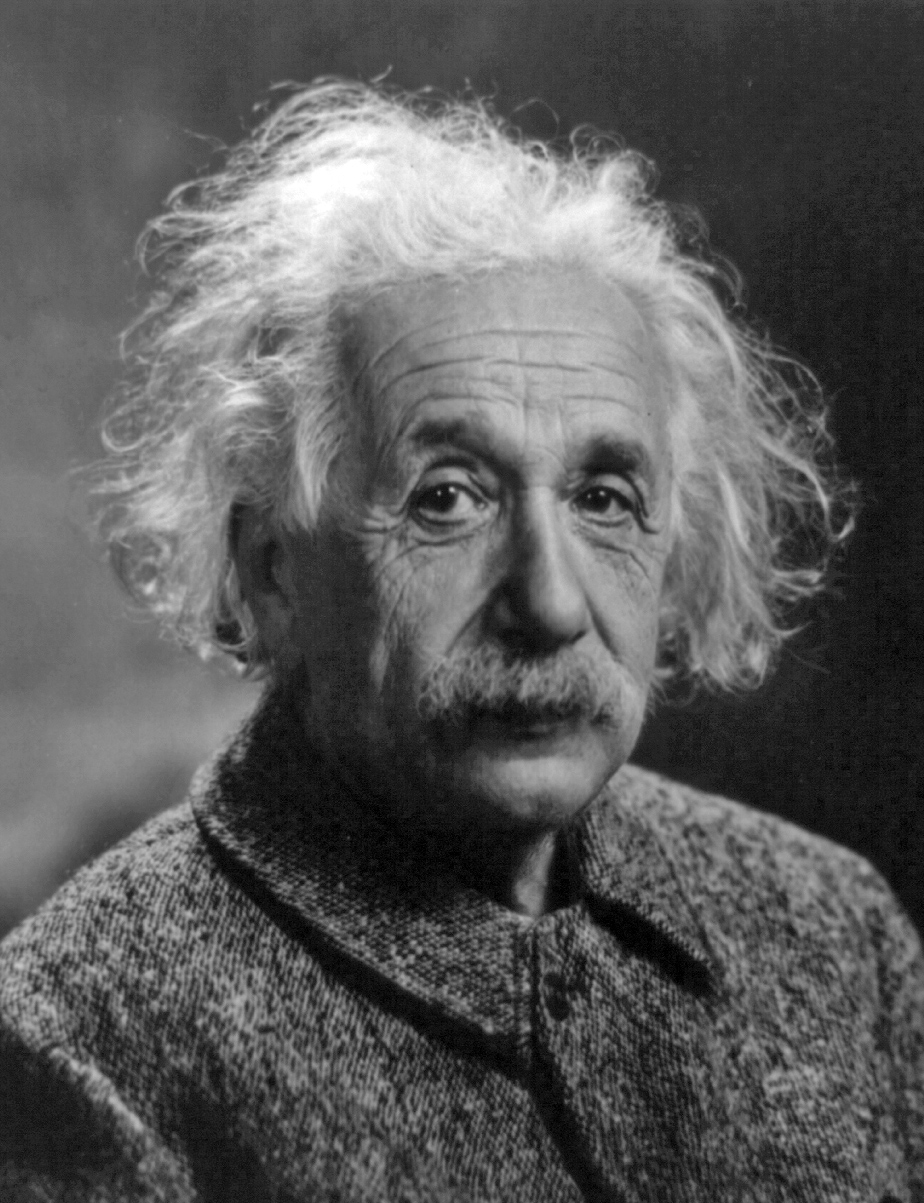
\includegraphics[height=35mm]{mypicture}}
\newcommand{\Photo}{}

\begin{document}
\title{Highlights of ATLAS Search Results}

\author{Bingxuan Liu, on behalf of the ATLAS Collaboration \footnote{Copyright CERN for the benefit of the ATLAS Collaboration. CC-BY-4.0 license}}

\address{Department of Physics, Simon Fraser University, Vancouver, Canada}

\maketitle\abstracts{Searching for beyond the standard model (BSM) physics has
been one of the primary goals of the Large Hadron Collider (LHC).  The LHC
delivered 140 $\mathrm{fb}^{-1}$ data of high quality in Run 2 for physics
analyses, allowing the ATLAS experiment to expand and improve its search
programme. The recent development in detector performance and analysis
techniques have brought significant boosts to the search sensitivities. In this
article, highlights of recent ATLAS search results are discussed and
summarised.}  

\section{Introduction}

Many mysteries in particle physics, such as the hierarchy problem, the origin
of dark matter (DM) and neutrino masses are still waiting for answers or hints
from the Large Hadron Collider (LHC). ATLAS has conducted a comprehensive set
of searches in the past years. Even though no evidence of BSM physics has been
reported, those searches excluded a large part of the phase space for many
models. For instance, the search for heavy particles in the di-jet final state
has explored the mass up to 8 TeV~\cite{dijet}. ATLAS has accumulated 140
$\mathrm{fb}^{-1}$ of high quality data for physics analyses in Run 2. It is
imperative to maximise its physics return. The searches discussed in this
article are categorised into three scenarios: searches upgrading previous
iterations using cutting-edge analysis techniques, searches filling the gaps
between explored regions of phase space, and searches considering challenging,
completely uncovered signatures.      

\section{Full Run 2 Upgrades of Previous Results}

The detector performance in ATLAS is continuously improving. For instance, the
performance of bottom- and top-tagging has advanced significantly in the past
few years. In addition, the application of machine learning techniques have
become very mature in physics analyses, enhancing the sensitivities. Even
though previous analyses have explored similar final states, the full Run-2
upgrades of those searches will push the exclusion limits further. Three new
search results are introduced in this section.\\

In the full Run 2 ATLAS vector-like quark search, the top partner masses with
50\% decay width are excluded up to 1975 GeV for the singlet representation~\cite{vlq},
considering $B(T\rightarrow Wb)=0.5$, as shown in
Figure~\ref{fig:limits1}\subref{fig:vlq}. Compared to the previous analysis
probing the same final state, this analysis adopted an updated top-tagger and
more optimised selections, achieving greatly improved sensitivities~\cite{vlq}.
The ATLAS full Run 2 right-handed neutrino search sets the most stringent
limits on the Keung-Senjanovi\'c process in the TeV $W$ partner
($W_{\mathrm{R}}$) mass region~\cite{rhn}. This search considers both the ``resolved'' and
``merged'' cases, depending on the mass split between the $W_{\mathrm{R}}$ and
the heavy neutrino ($N_{\mathrm{R}}$). The ``resolved'' case uses well
separated reconstructed objects while the ``merged'' case utilises a single object
formed by several nearby objects. For Majorana neutrinos, in the muon channel,
the limit on $m(W_{\mathrm{R}})$ reaches 6.4 TeV for $m(N_{\mathrm{R}})=1$ TeV,
and the limit on $m(N_{\mathrm{R}})$ extends to 3.6 TeV for
$m(W_{\mathrm{R}})=4.8$ TeV, as shown in
Figure~\ref{fig:limits1}\subref{fig:rhn}~\cite{rhn}.\\           

The combination of different analyses offers a powerful way to constrain a given
type of model. A recent ATLAS search is concentrated on final states with
$\tau$ leptons and hadronic jets, providing interpretation including both the
leptoquark (LQ) and excited $\tau$ models~\cite{tau}. In particular, it is sensitive to
$LQ\rightarrow c\tau^{-}$ ($\overline{LQ}\rightarrow\overline{c}\tau^{+}$)
decays, as the analysis does not require any jets to be $b$-tagged. It
comprises a critical piece in the leptoquark combination given this unique
feature of the signal region selection. Masses below 1.3 TeV are excluded,
assuming the branching ratio of their decays to the $c$-quark-$\tau$-lepton
pair is equal to one~\cite{tau}.\\   

\begin{figure}[htp]
     \centering
     \begin{subfigure}[b]{0.35\textwidth}
         \centering
         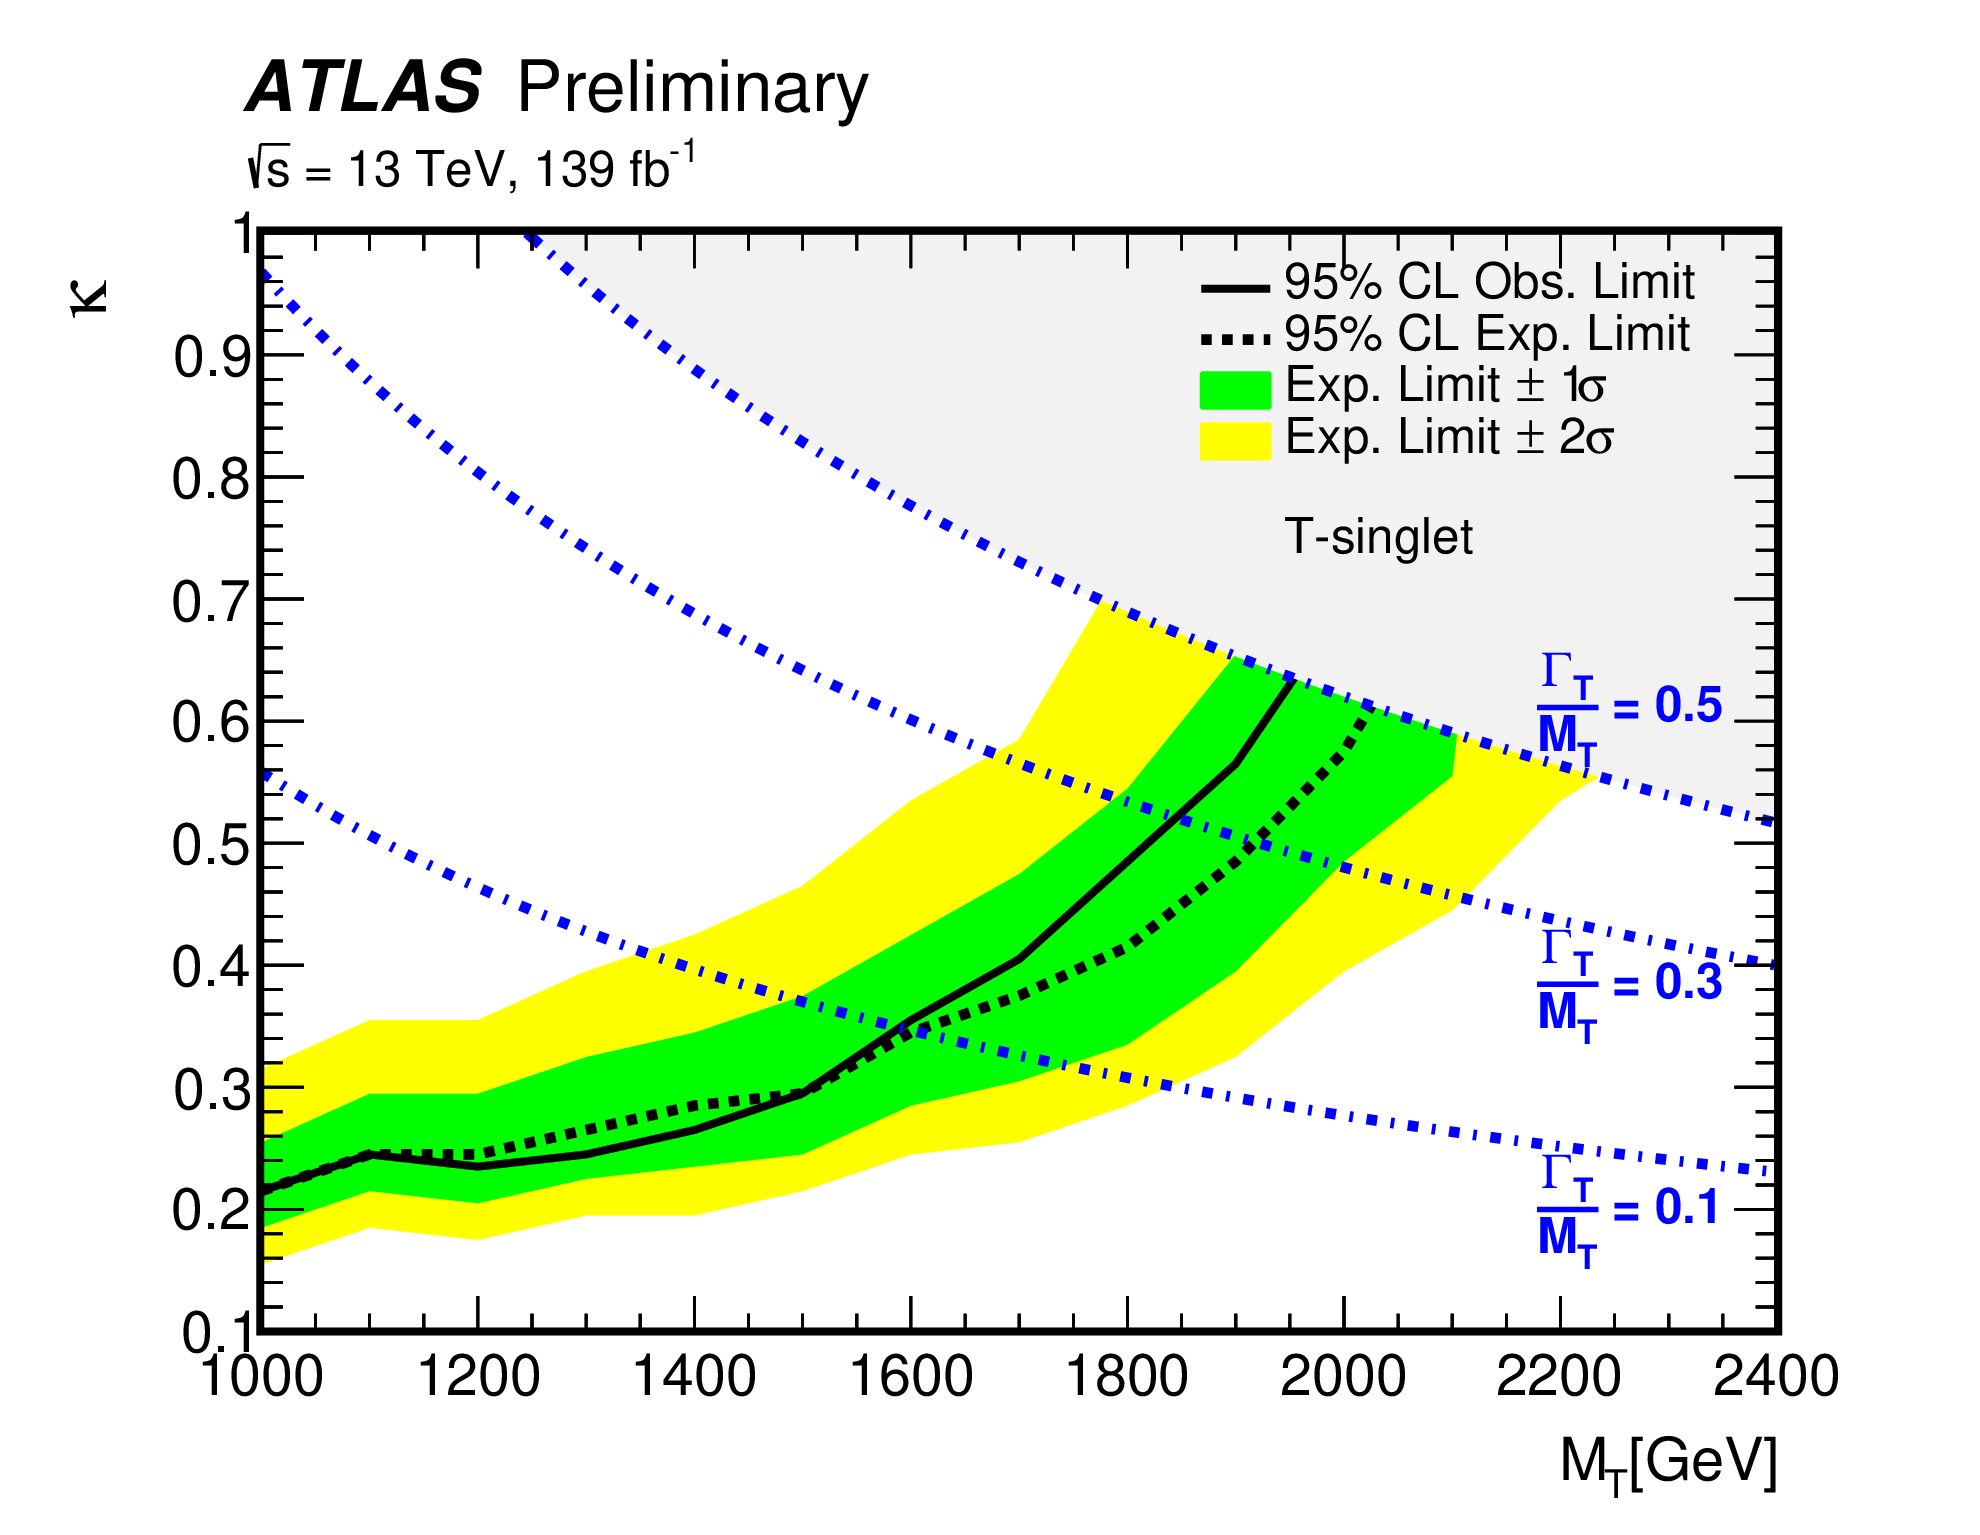
\includegraphics[width=\textwidth]{VLQ}
         \caption{}
         \label{fig:vlq}
     \end{subfigure}
     \begin{subfigure}[b]{0.32\textwidth}
         \centering
         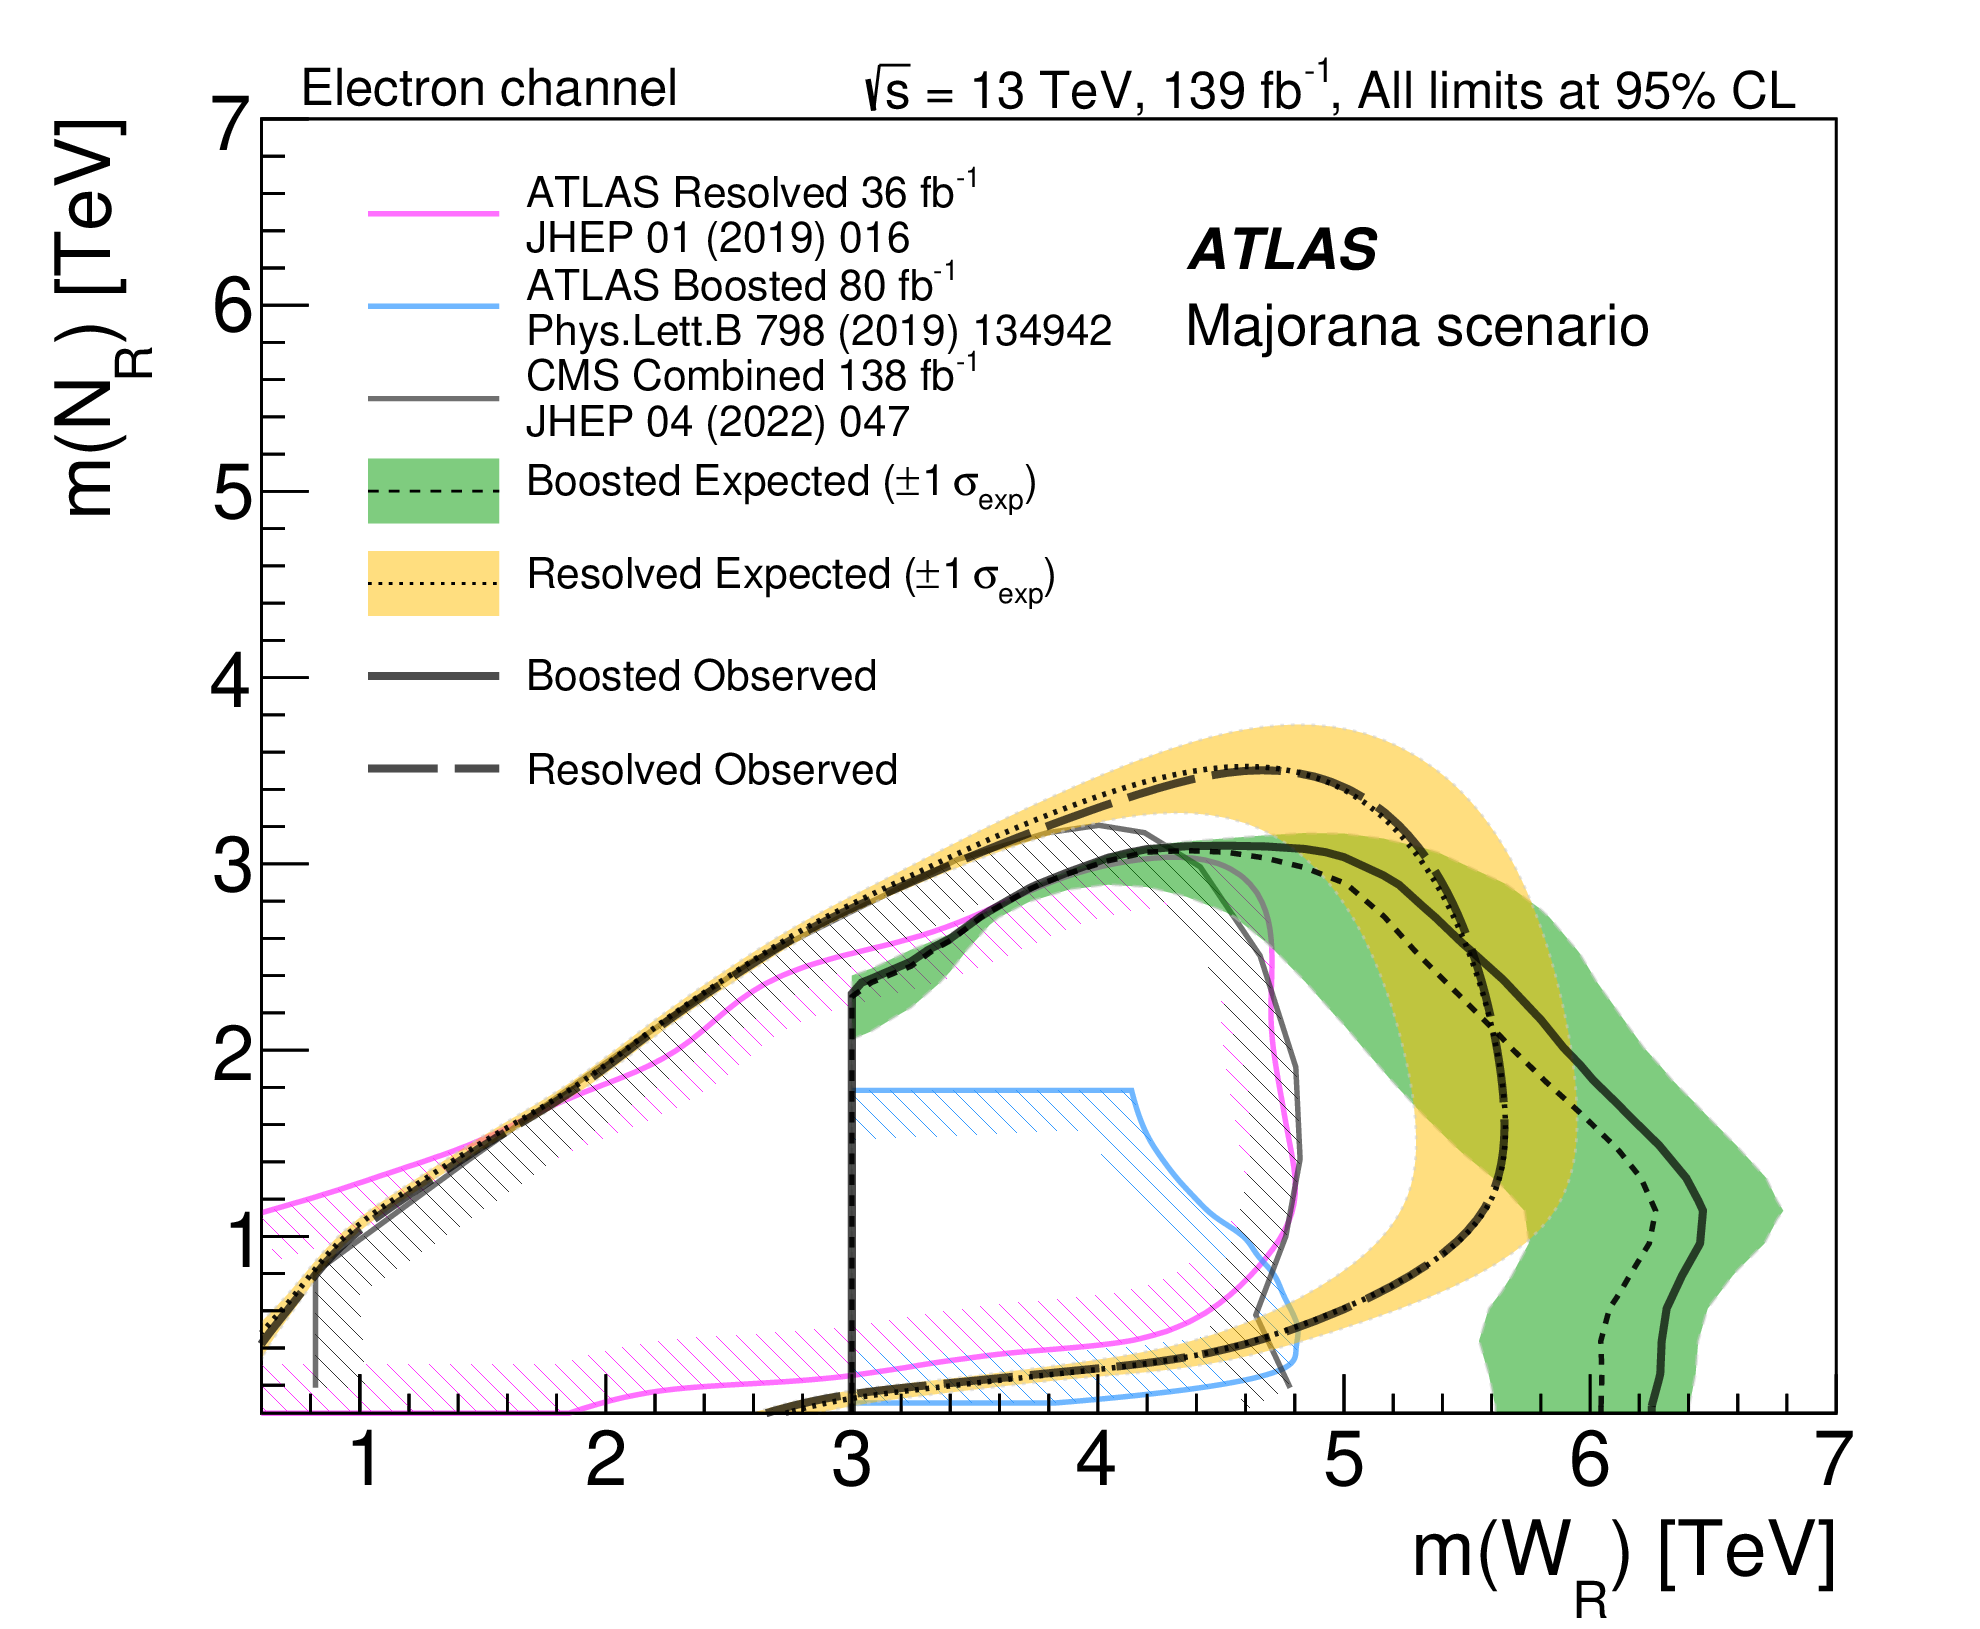
\includegraphics[width=\textwidth]{RHN}
         \caption{}
         \label{fig:rhn}
     \end{subfigure}
     \caption{Observed (solid line) and expected (dashed line) limits or contours on: (a) the singlet representation of a vector like top-quark\protect\cite{vlq}; (b) Majorana heavy neutrino on the $m(W_{\mathrm{R}})-m(N_{\mathrm{R}})$ mass plane\protect\cite{rhn}.}
     \label{fig:limits1}
\end{figure}

\section{Dedicated Searches to Cover the Unexplored Regions}

There have been many well motivated BSM models proposed by the theory community
in the past decades. The number of free parameters in those models can be so
large that a single search can only probe a subset of the parameter space and a
particular combination of masses or couplings. Naturally, there are gaps
between existing searches, and they have to be explored as new physics can hide
there. The gap regions are usually hard to study so that special analysis
strategies are essential.\\

In the realm of supersymmetry searches, there are various uncovered corners on
specific parameter planes that are quite challenging. A recent ATLAS search for
higgsinos considers the $b\overline{b}\gamma\gamma$ final state, taking
advantage of the excellent mass resolution of the photons and the large
$H\rightarrow b\overline{b}$ branching ratio~\cite{bbyy}. It successfully fills the gap in
the low mass region, as seen in Figure
~\ref{fig:limits2}\subref{fig:bbyy}~\cite{bbyy}.\\

The gap between dedicated long-lived particle (LLP) searches and searches only
considering prompt signatures is becoming increasingly important. A recent
ATLAS search for micro-displaced muons is focused on this gap region using
muons reconstructed by the standard algorithms, requiring the transverse impact
parameter ($|d_{0}|$) of the muons to be between 0.1 and 3 mm. Control regions,
validation regions, and signal regions are constructed using the muon $|d_{0}|$
and muon-pair mass.  In the context of a smuon pair production, the gap between
the conventional search and the dedicated LLP search is filled, as shown in
Figure ~\ref{fig:limits2}\subref{fig:micro}~\cite{micro}.\\   

Certain BSM models should be searched in various experiments. For instance, in models considering the
hidden sectors, the dark photon mass can vary from MeV to TeV. A recent
ATLAS search looks for dark photons in the 4$l$ + $X$ final state, where the
four leptons are from two dark photons ($A'$). The average invariant mass of
the two lepton pairs is used as the main observable. The four-lepton mass is
used to construct signal and control regions, while the lepton pair mass is
used to suppress quarkonia background.  This search excludes the much higher
mass region compared to the results from the Belle collaboration~\cite{dark}.\\

\begin{figure}[htp]
     \centering
     \begin{subfigure}[b]{0.35\textwidth}
         \centering
         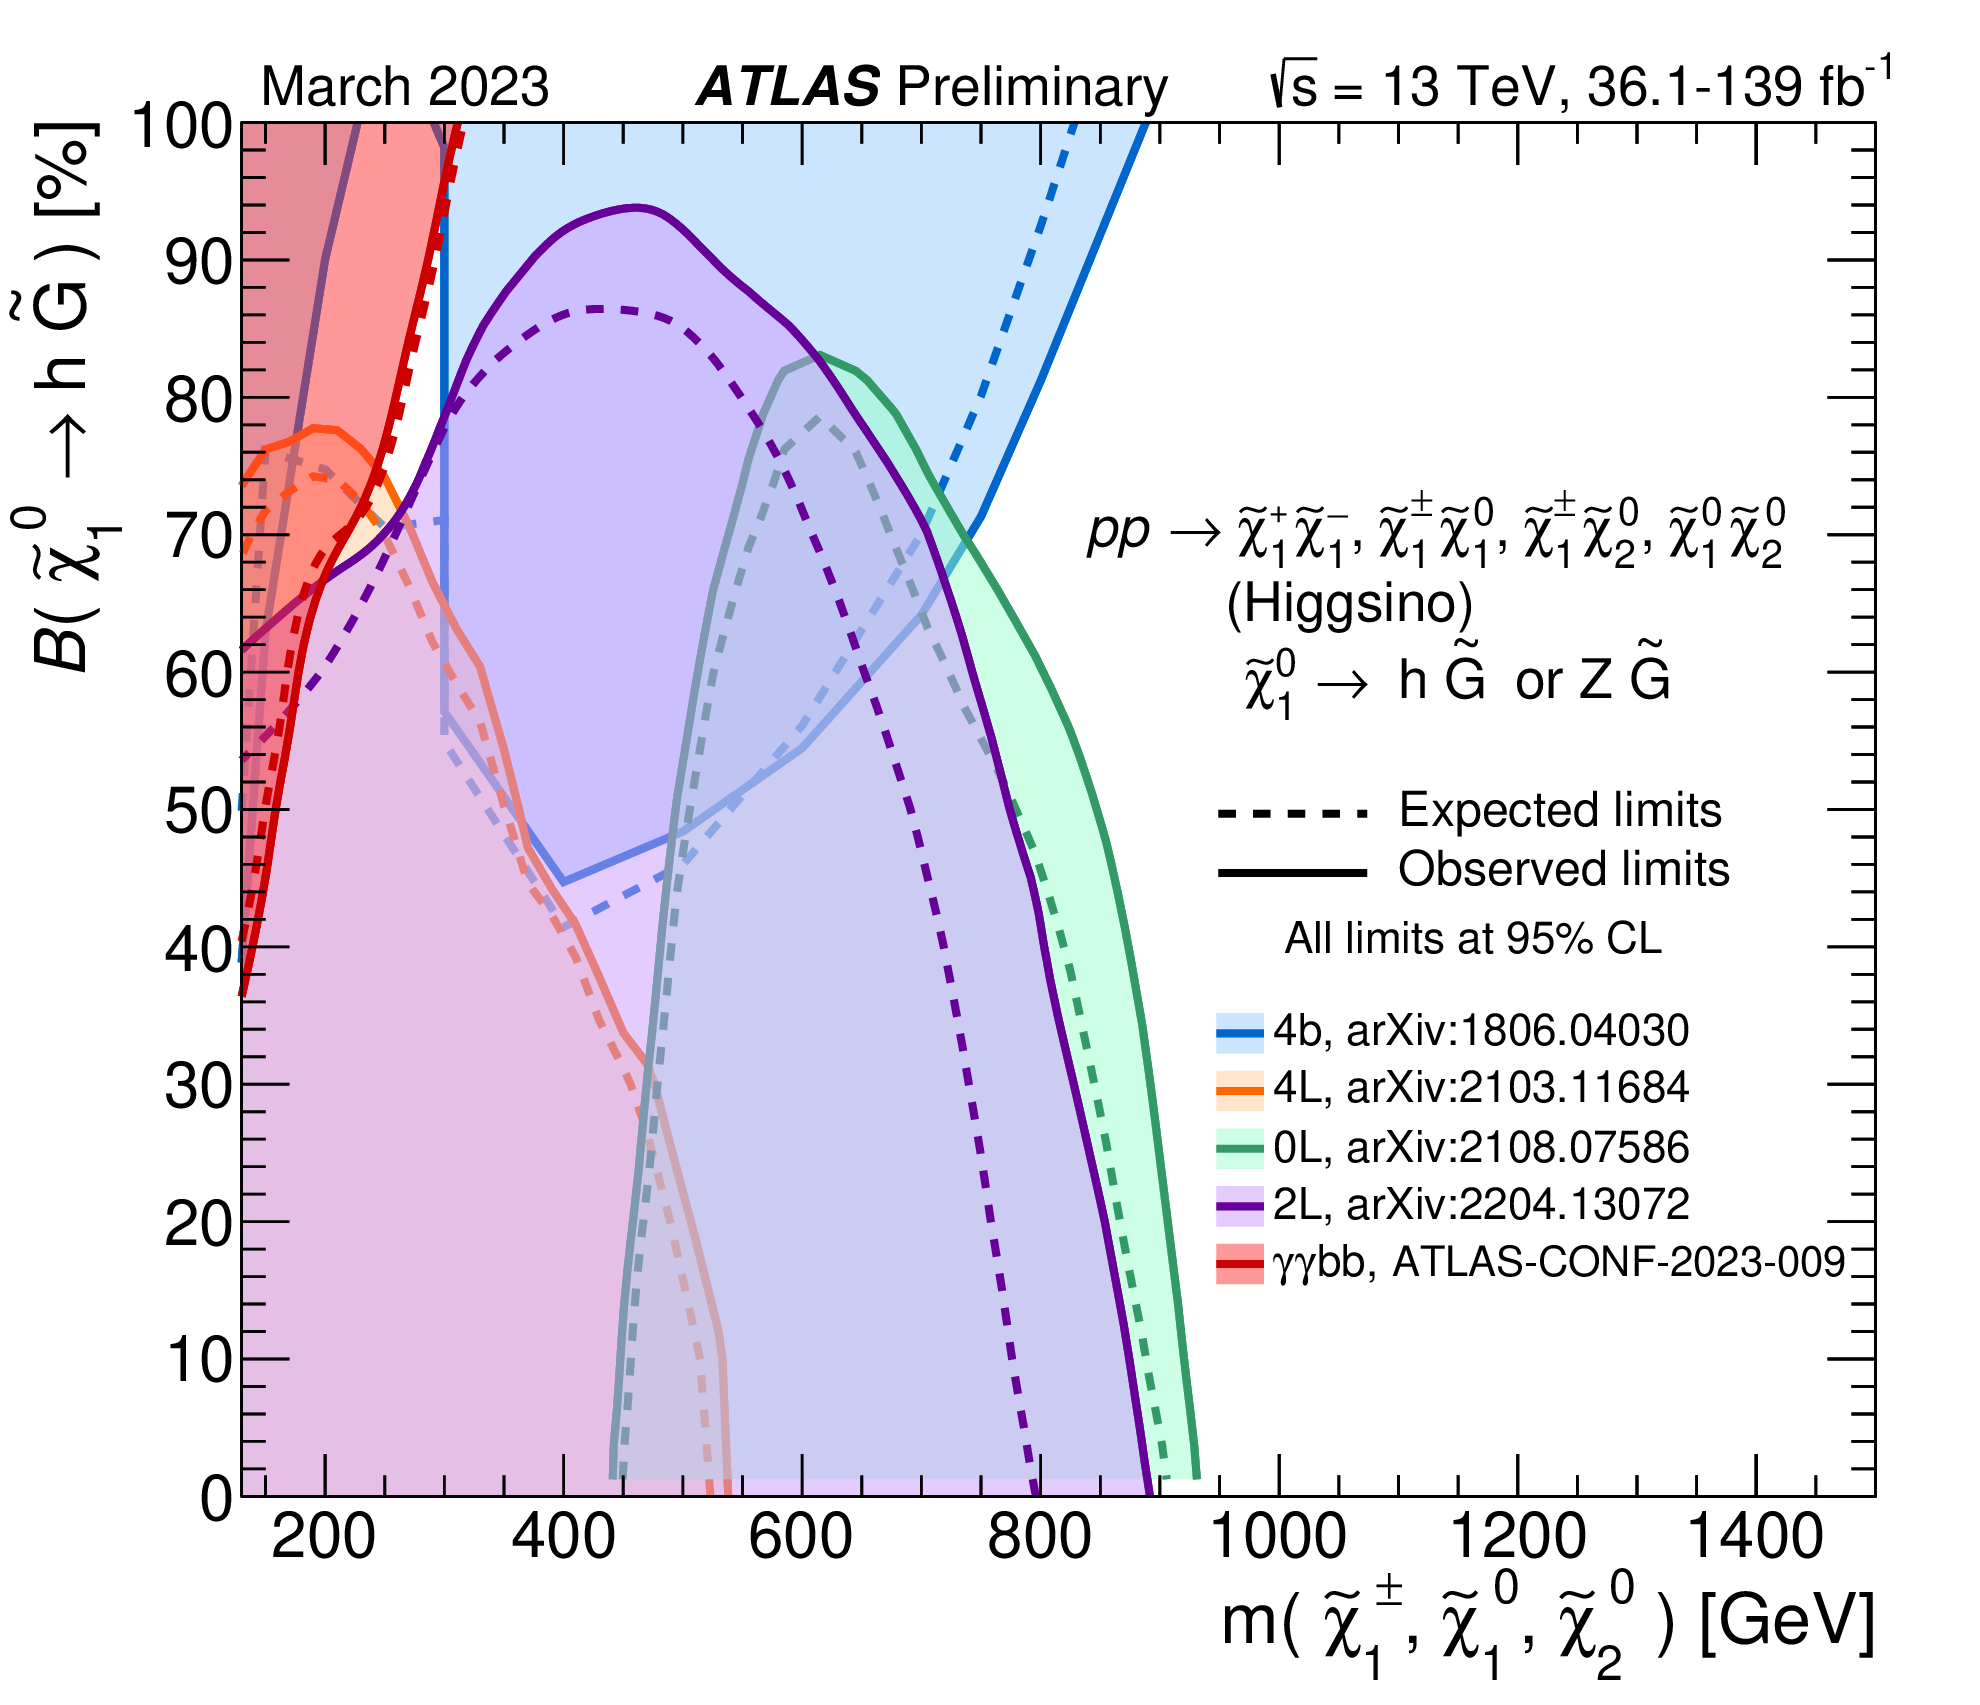
\includegraphics[width=\textwidth]{bbyy}
         \caption{}
         \label{fig:bbyy}
     \end{subfigure}
     \begin{subfigure}[b]{0.32\textwidth}
         \centering
         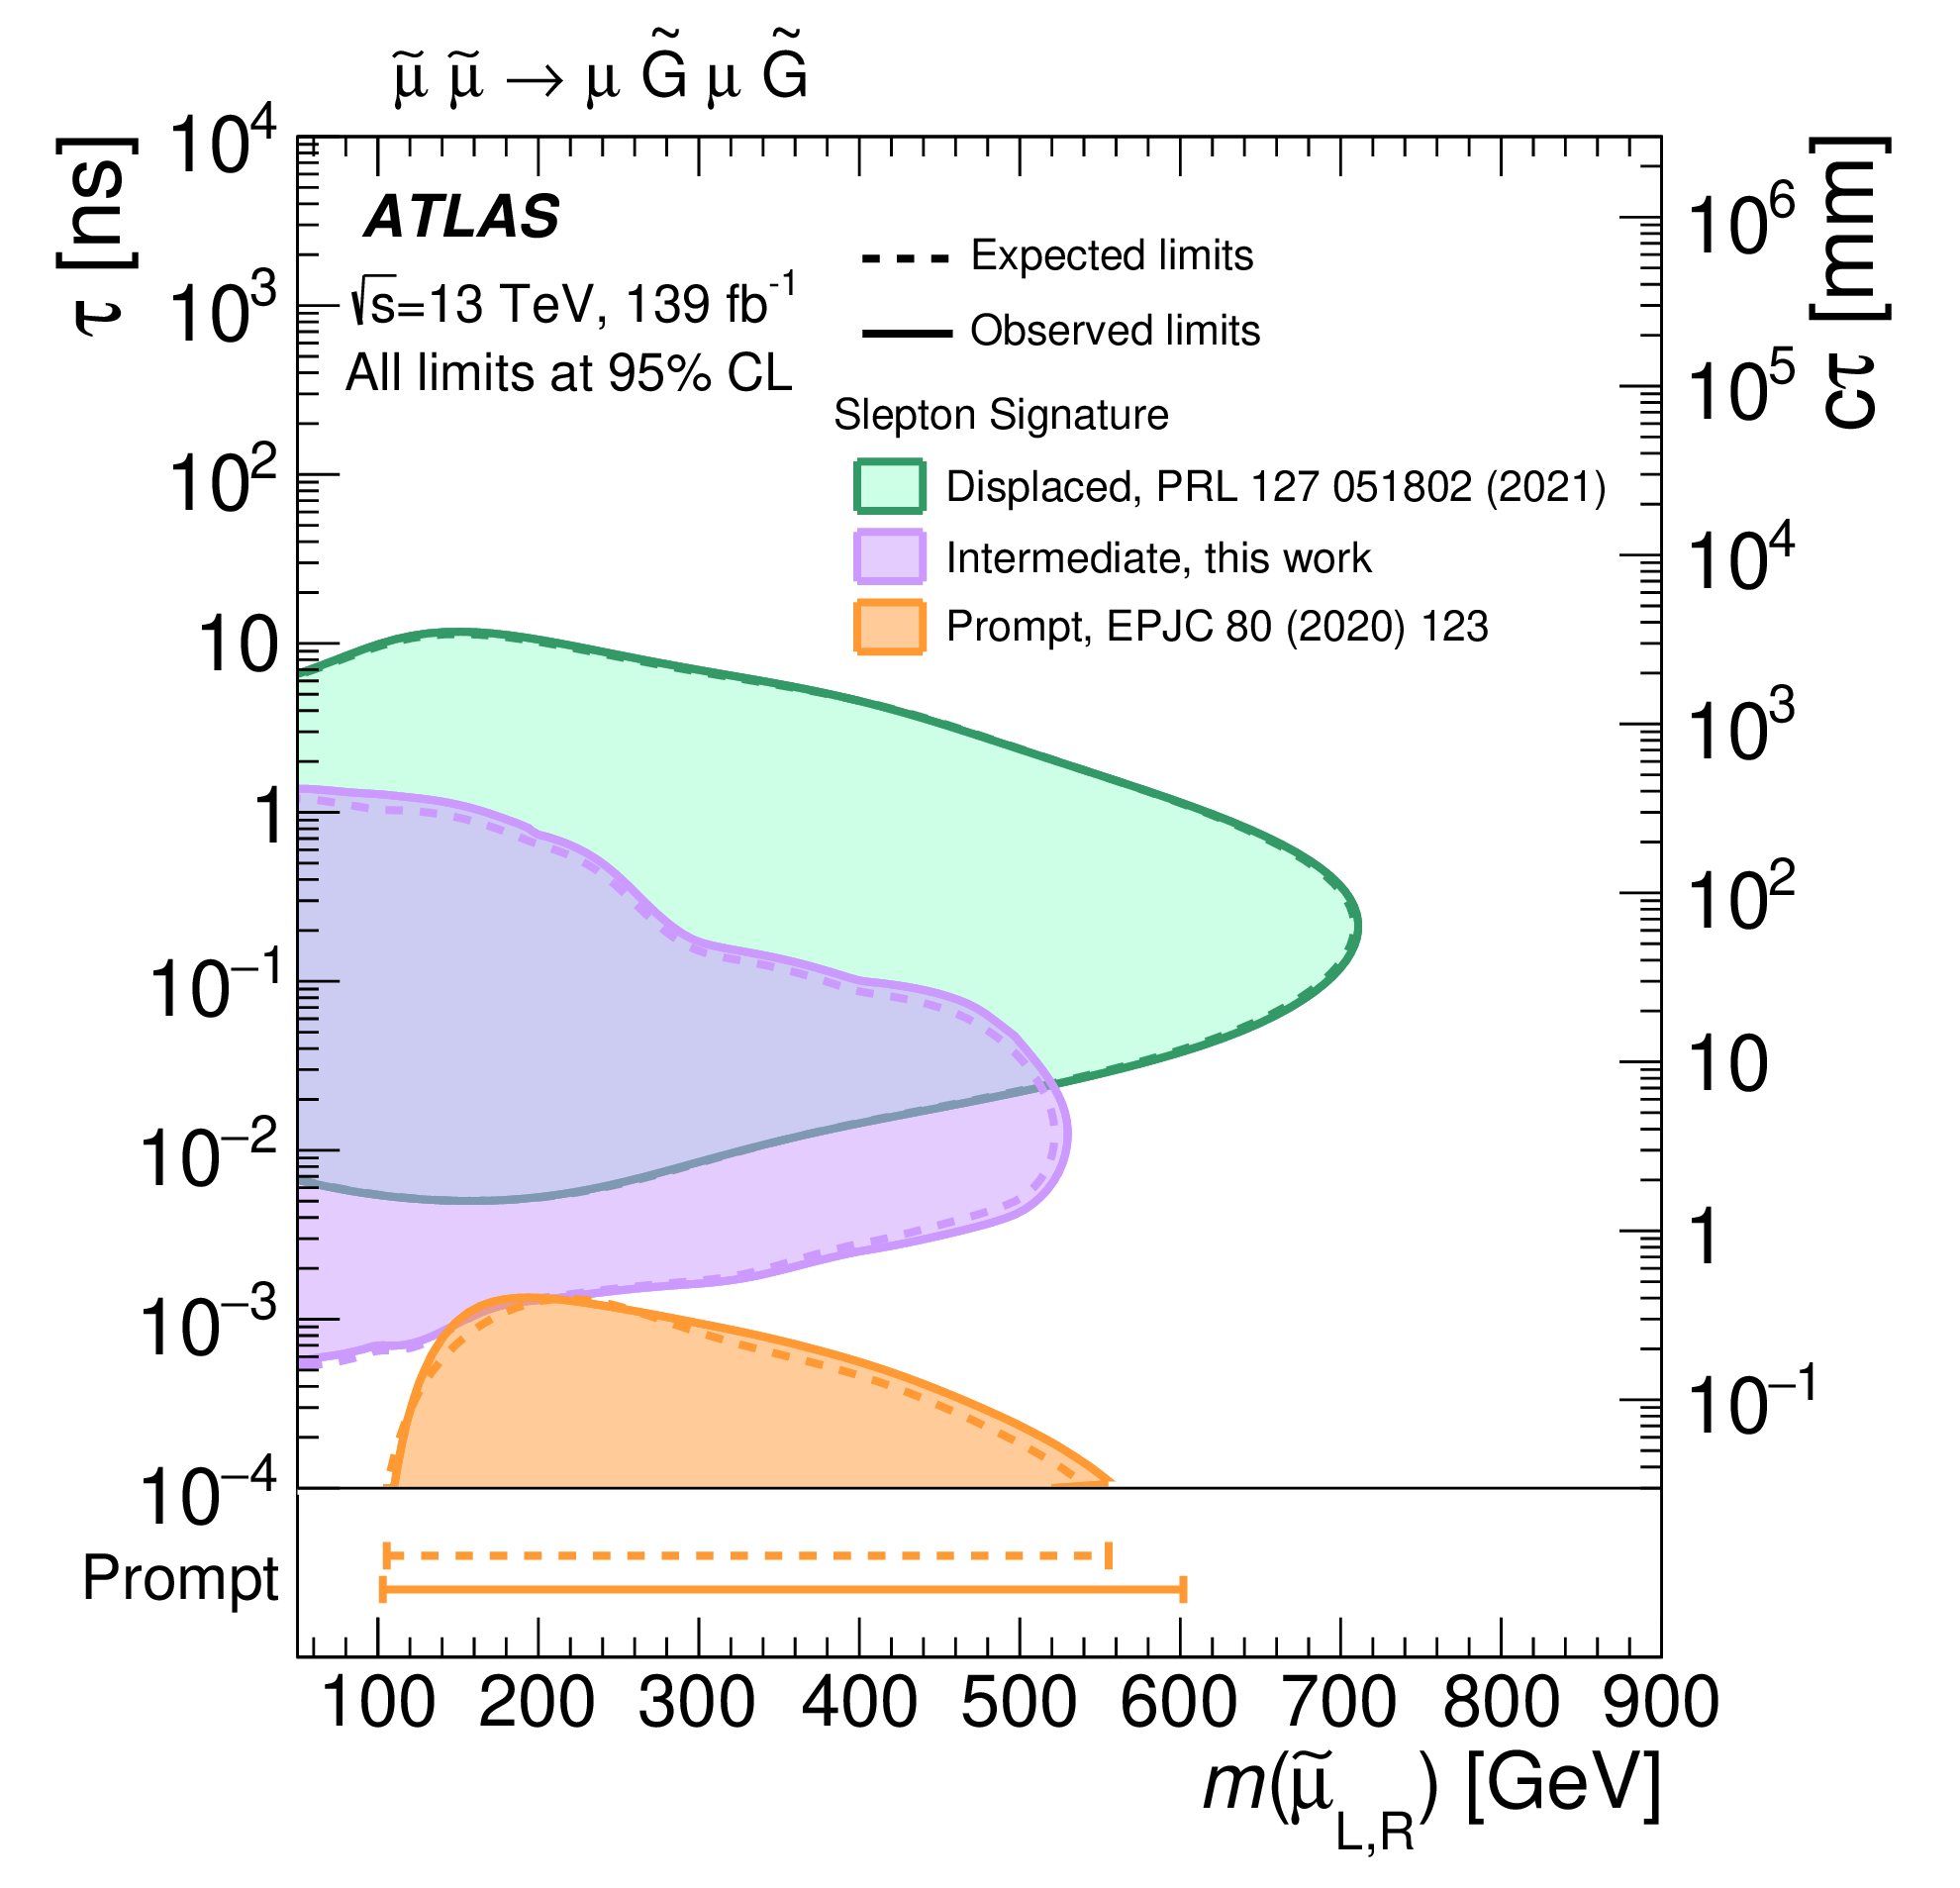
\includegraphics[width=\textwidth]{micro}
         \caption{}
         \label{fig:micro}
     \end{subfigure}
        \caption{(a): Exclusion contour of the higgsino pair production on the mass and branching ratio 2D plane\protect\cite{bbyy}. (b): Exclusion contour of the smuon pair production on the mass and lifetime 2D plane\protect\cite{micro}.}
        \label{fig:limits2}
\end{figure}

\section{Searches for New and Challenging Signatures}

ATLAS is capable of studying an impressive amount of signatures, but there are
signatures known to be very challenging. A signature can be strenuous because
the traditional analysis techniques are not suitable. Analyses challenging
those signatures can greatly broaden the ATLAS search programme. Two new
searches will be covered in this section.\\

ATLAS has searched for heavy particles produced in association with two
top-quarks, decaying to two top-quarks, i.e., top-philic heavy particles. The
previous search considered the non-resonant production as the reconstructed
$t\overline{t}$ mass is very broad as seen in
Figure~\ref{fig:tttt}\subref{fig:mass}. A recent ATLAS analysis takes the
resonant production channel into account. A hybrid background estimation method
is developed to overcome the difficulties in dealing with broad signals. A
background template is obtained in an inclusive region first and then
propagated to the signal region via simulation, in order to minimize the biases
introduced by the broad signals. A global deviation scan is done first in a
model agnostic way, observing no significant deviations from the background in
data. The observed
(expected) limits on the production cross-section range from 21 (14) fb to 119
(86) fb depending on the choice of model parameters, shown in
Figure~\ref{fig:tttt}\subref{fig:ttttlimits}. The results are limited by the
modeling uncertainties~\cite{tttt}.\\    

\begin{figure}[htp]
     \centering
     \begin{subfigure}[b]{0.35\textwidth}
         \centering
         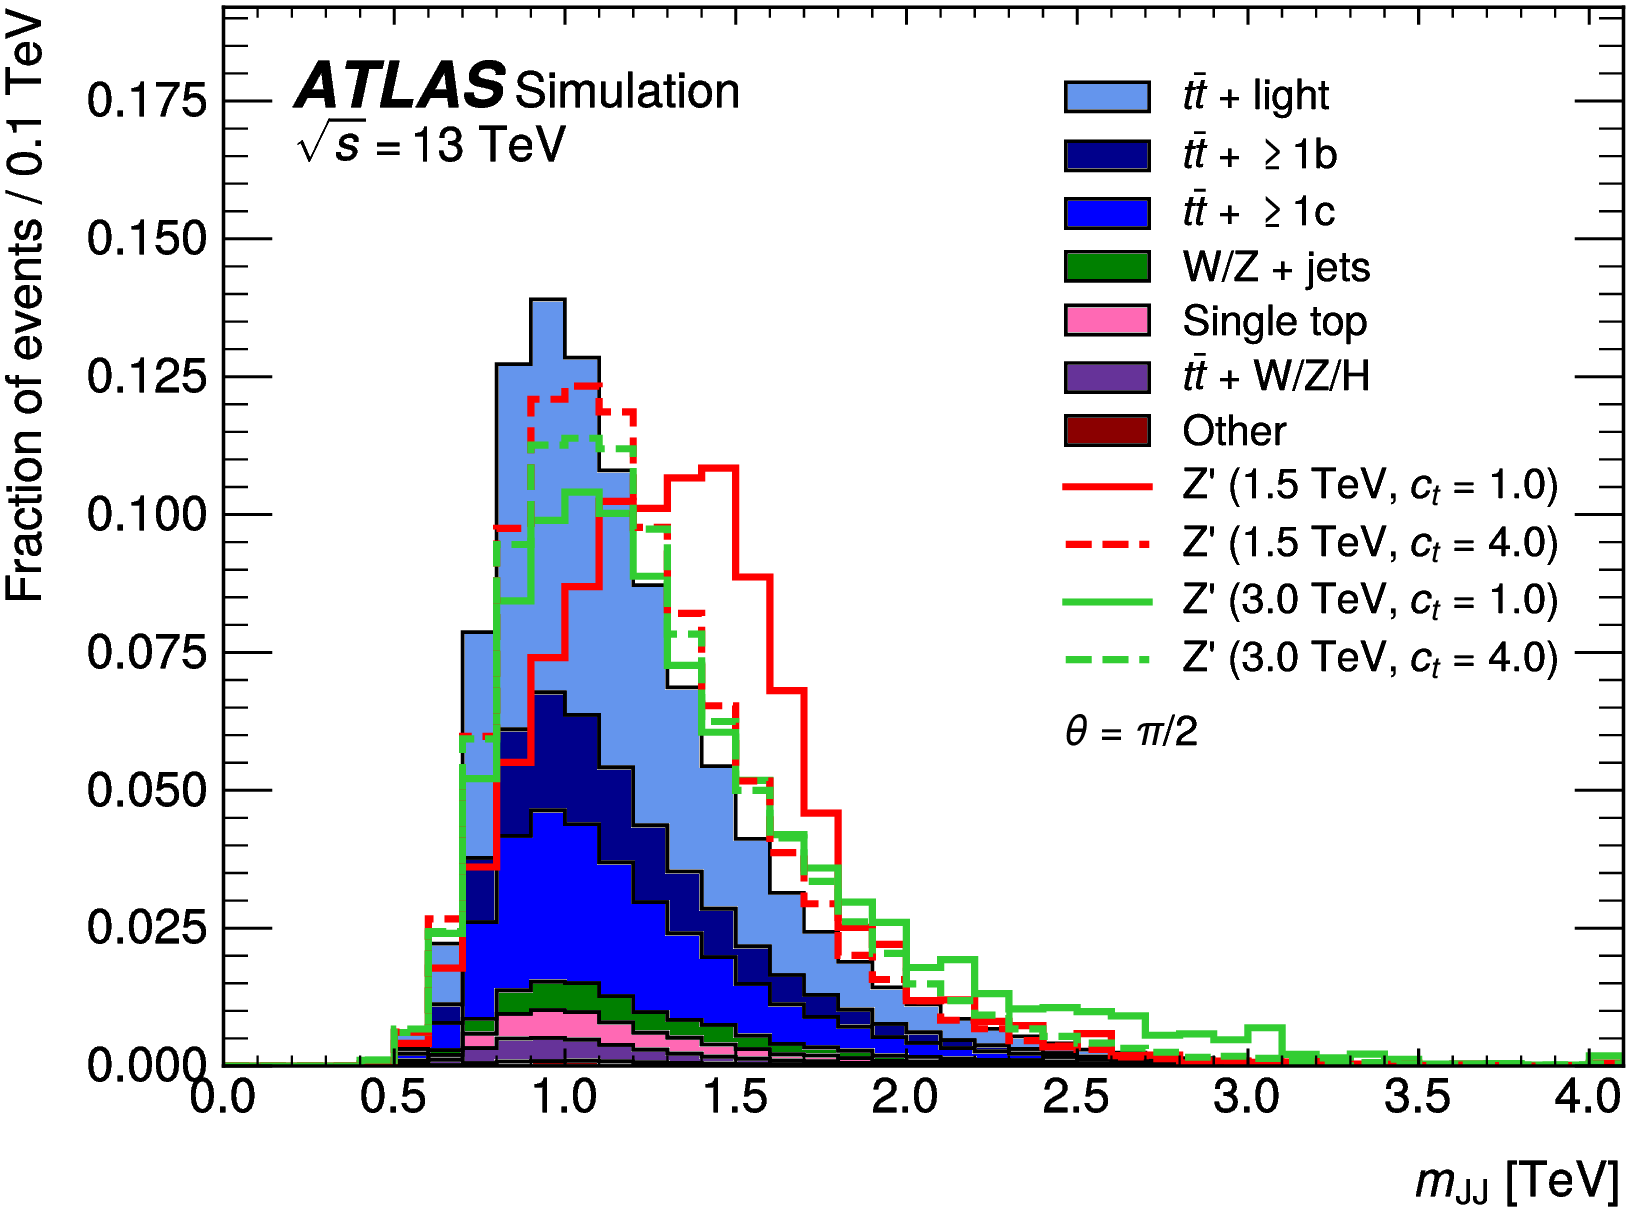
\includegraphics[width=\textwidth]{mass}
         \caption{}
         \label{fig:mass}
     \end{subfigure}
     \begin{subfigure}[b]{0.28\textwidth}
         \centering
         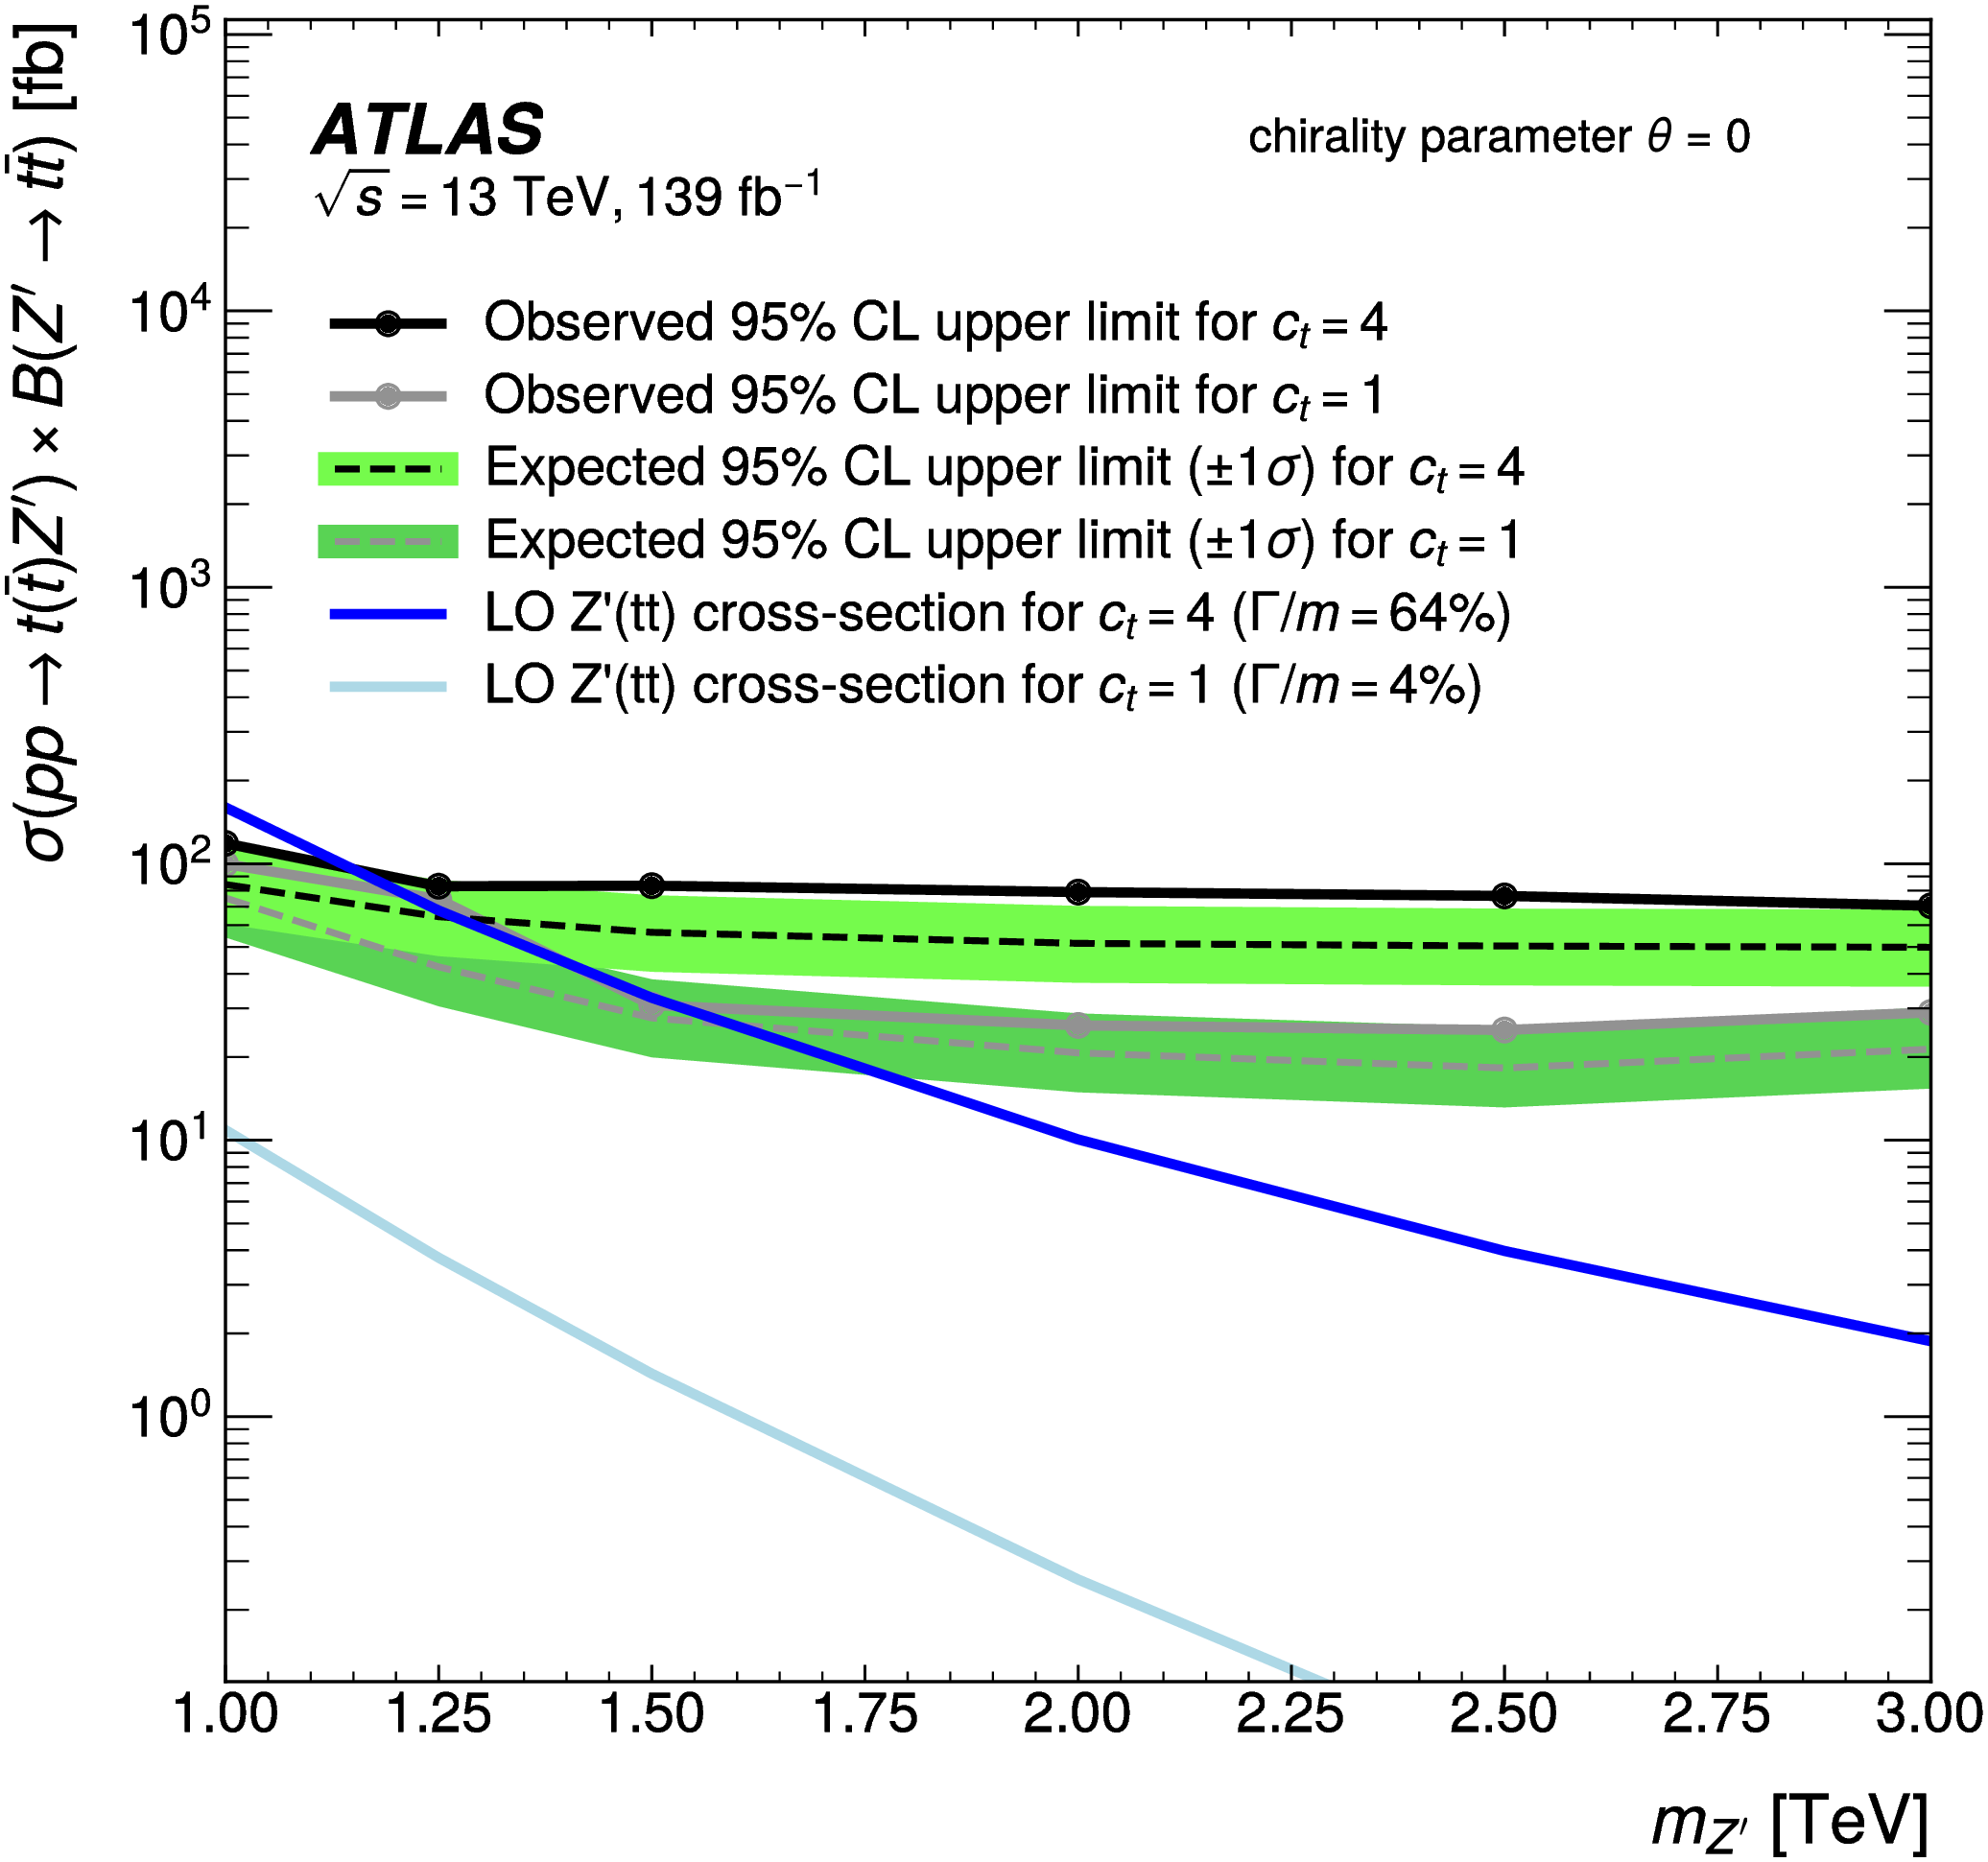
\includegraphics[width=\textwidth]{tttt}
         \caption{}
         \label{fig:ttttlimits}
     \end{subfigure}
        \caption{(a): Invariant mass distributions of the two large-R jets for different backgrounds and signal points. (b): Observed (solid line) and expected (dashed line) limits on the top-philic heavy particles as a function of mass\protect\cite{tttt}.}
        \label{fig:tttt}
\end{figure}

Searches are typically performed using conventional observables such as the
invariant mass as the one discussed above. A recent ATLAS search explores
periodic signals for the first time. Such a signal is predicted in the
clockwork (CW) or linear dilation (LD) framework~\cite{clock}. Instead of
having one peak in the invariant mass spectrum, these models predict continuous
narrow peaks, as illustrated in Figure~\ref{fig:periodic}\subref{fig:signal}.
The analysis applied a ``continuous wavelet'' transformation to the data
sample. A sample containing signal events creates an ``island'' on the
scalogram as depicted in Figure ~\ref{fig:periodic}\subref{fig:shape}. Limits
are set for the gravity scale, $M_{5}$, and the turn-on mass scale, $k$, shown
in Figure ~\ref{fig:periodic}\subref{fig:perlimits}~\cite{period}.  This search
has not only pioneered in probing this intriguing signature, but also
demonstrated that the data can be analyzed in a different space.\\        

\begin{figure}[htp]
     \centering
     \begin{subfigure}[b]{0.30\textwidth}
         \centering
         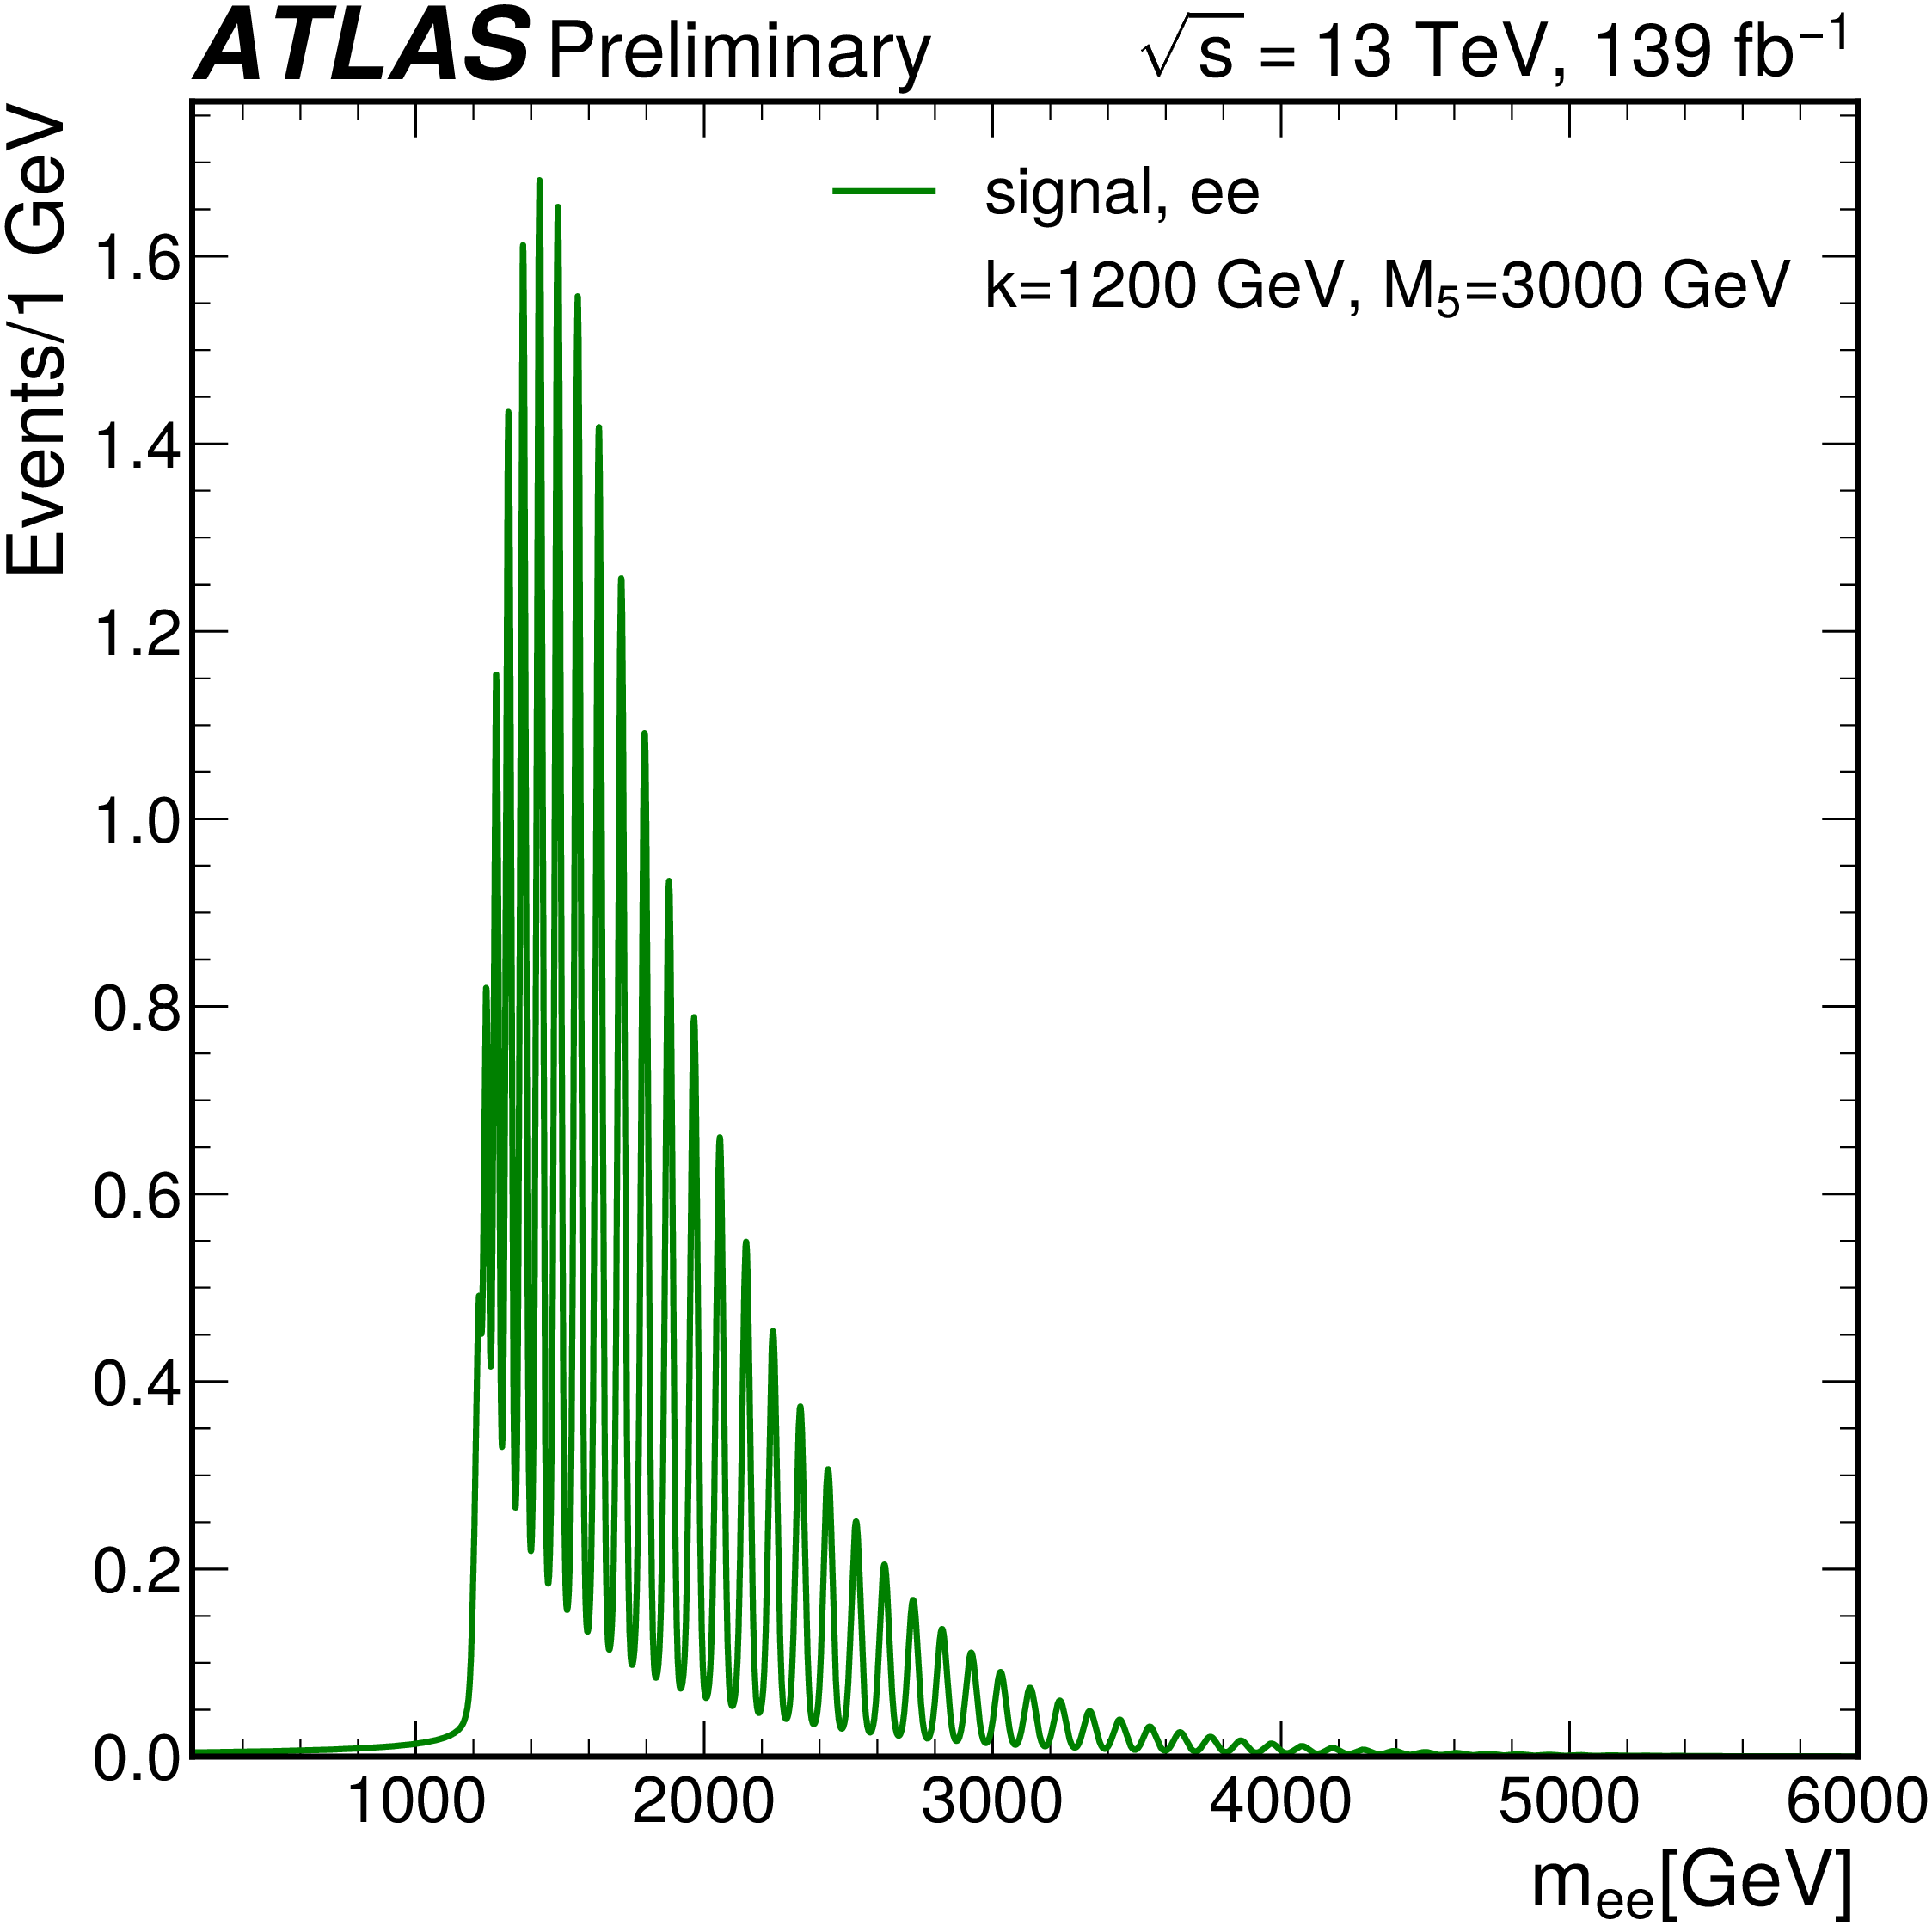
\includegraphics[width=\textwidth]{signal}
         \caption{}
         \label{fig:signal}
     \end{subfigure}
     \begin{subfigure}[b]{0.30\textwidth}
         \centering
         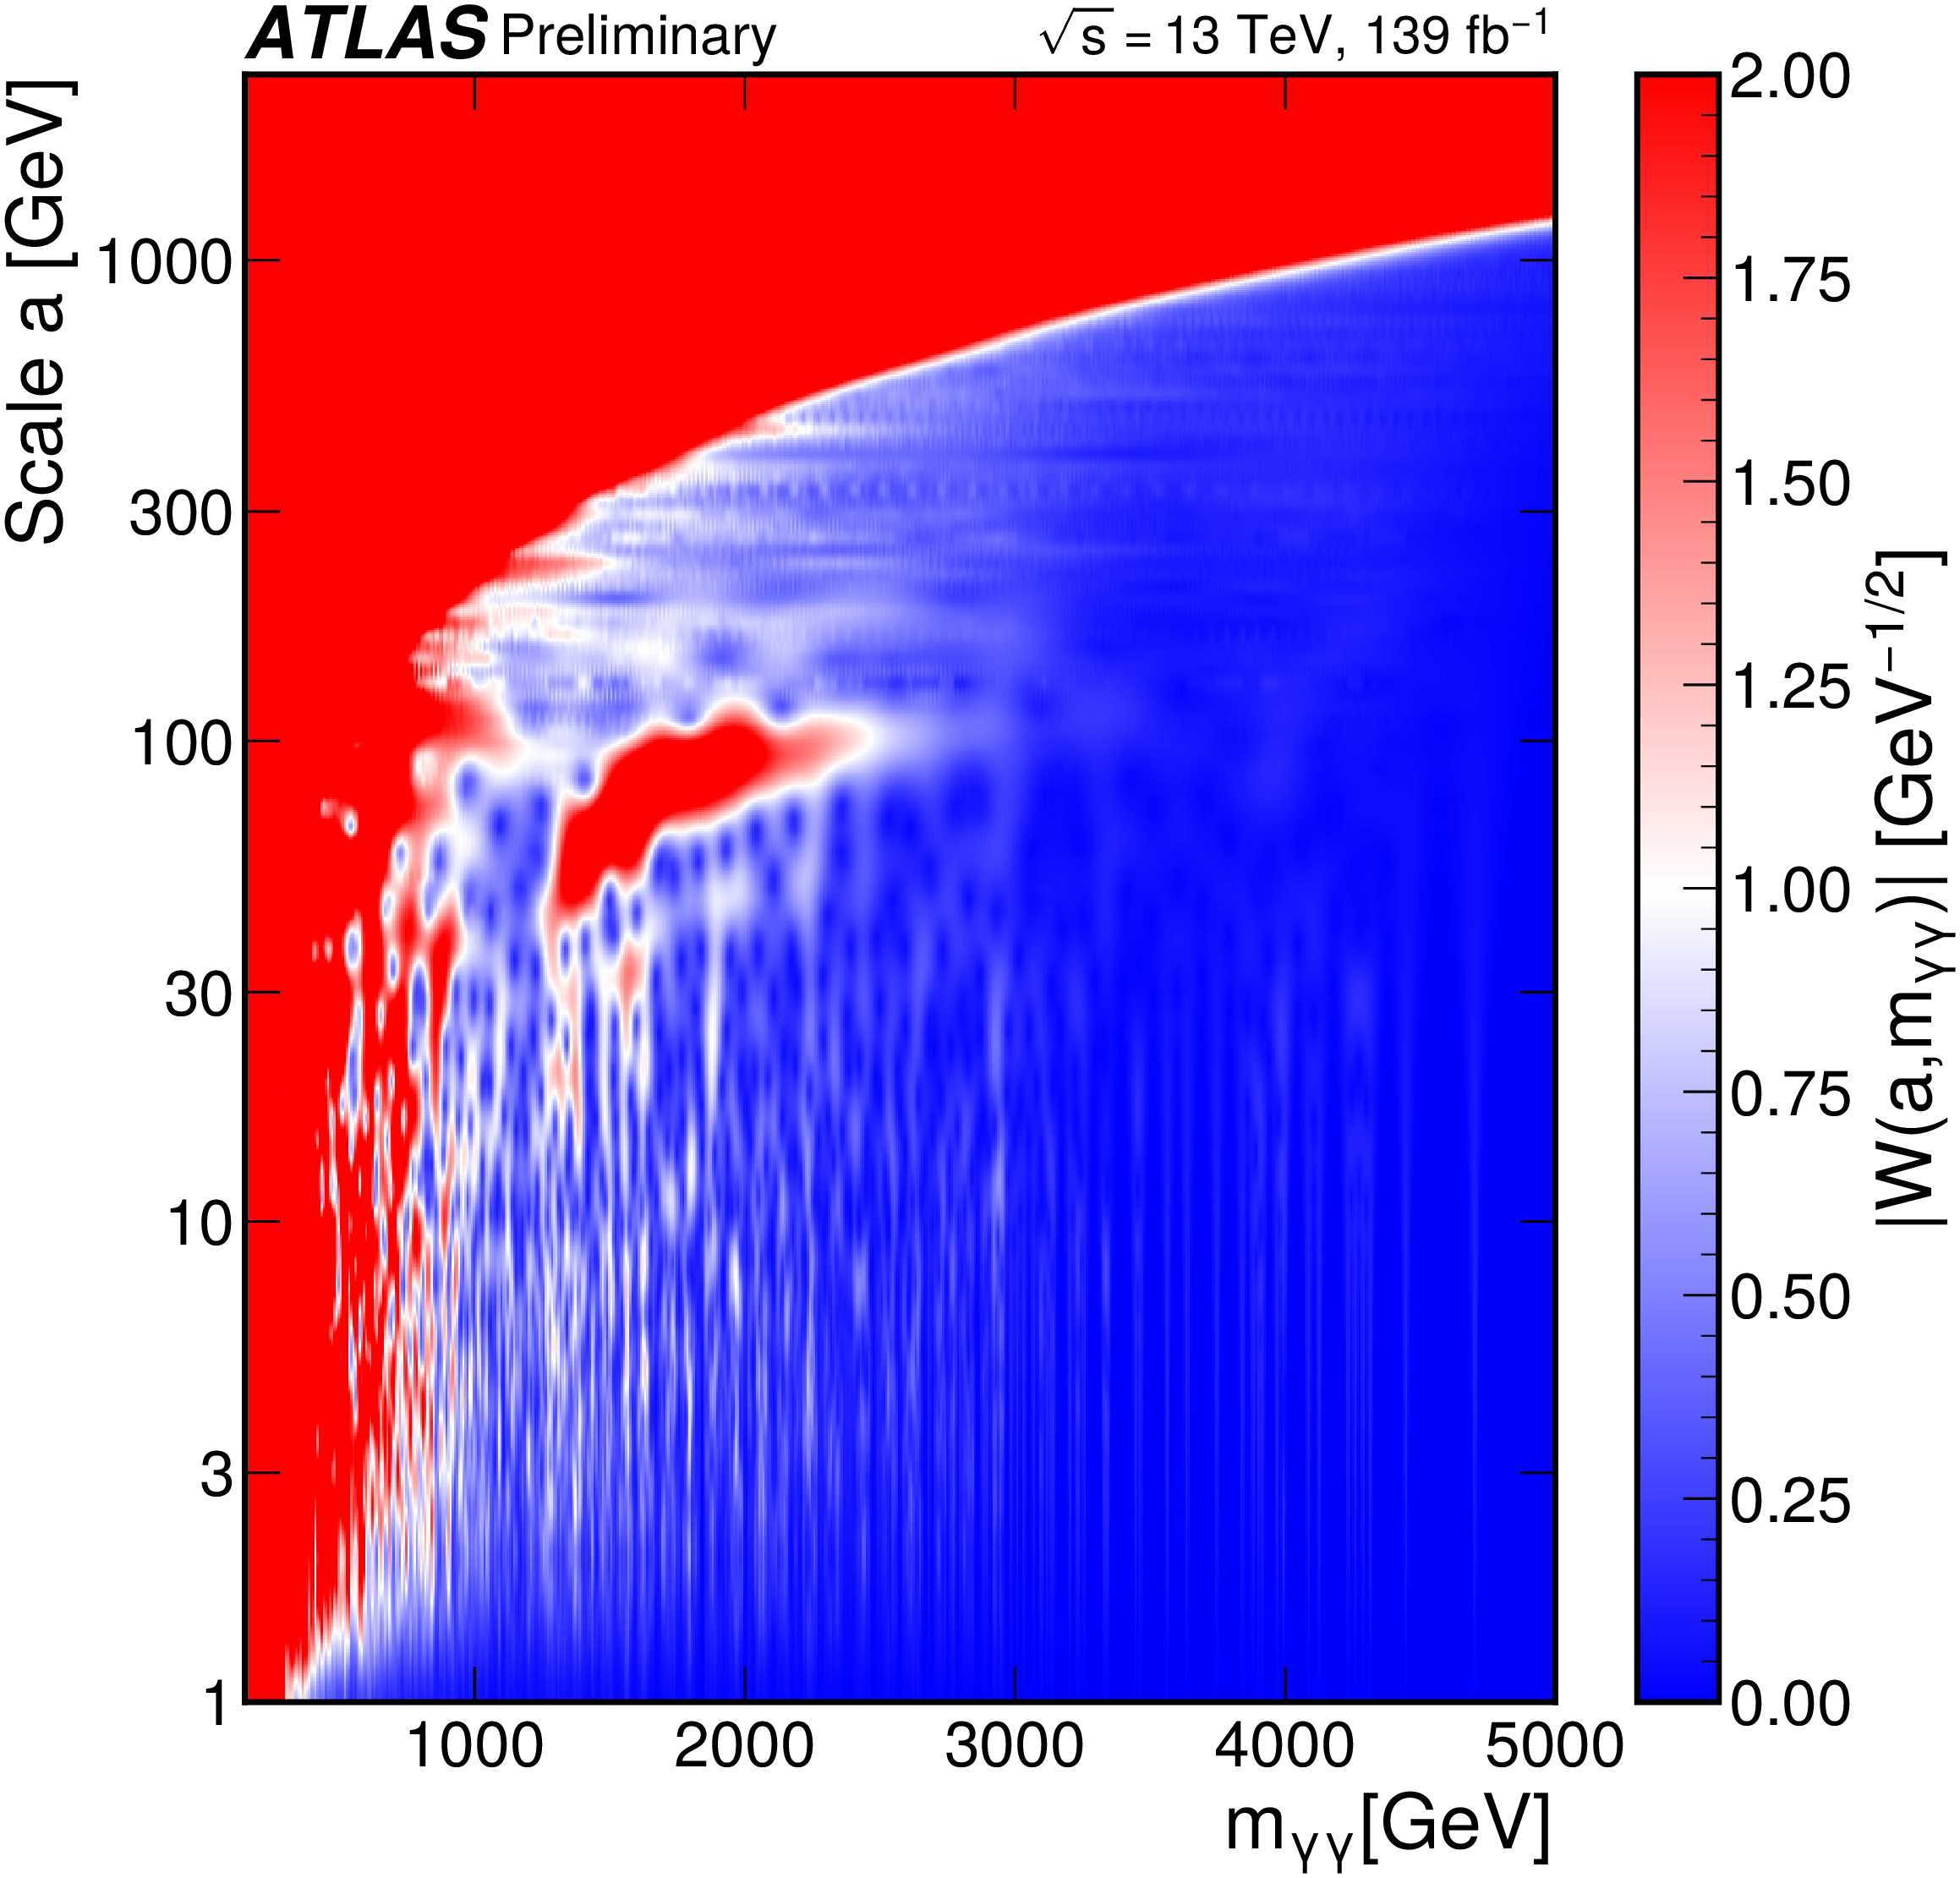
\includegraphics[width=\textwidth]{bkgsig}
         \caption{}
         \label{fig:shape}
     \end{subfigure}
     \begin{subfigure}[b]{0.30\textwidth}
         \centering
         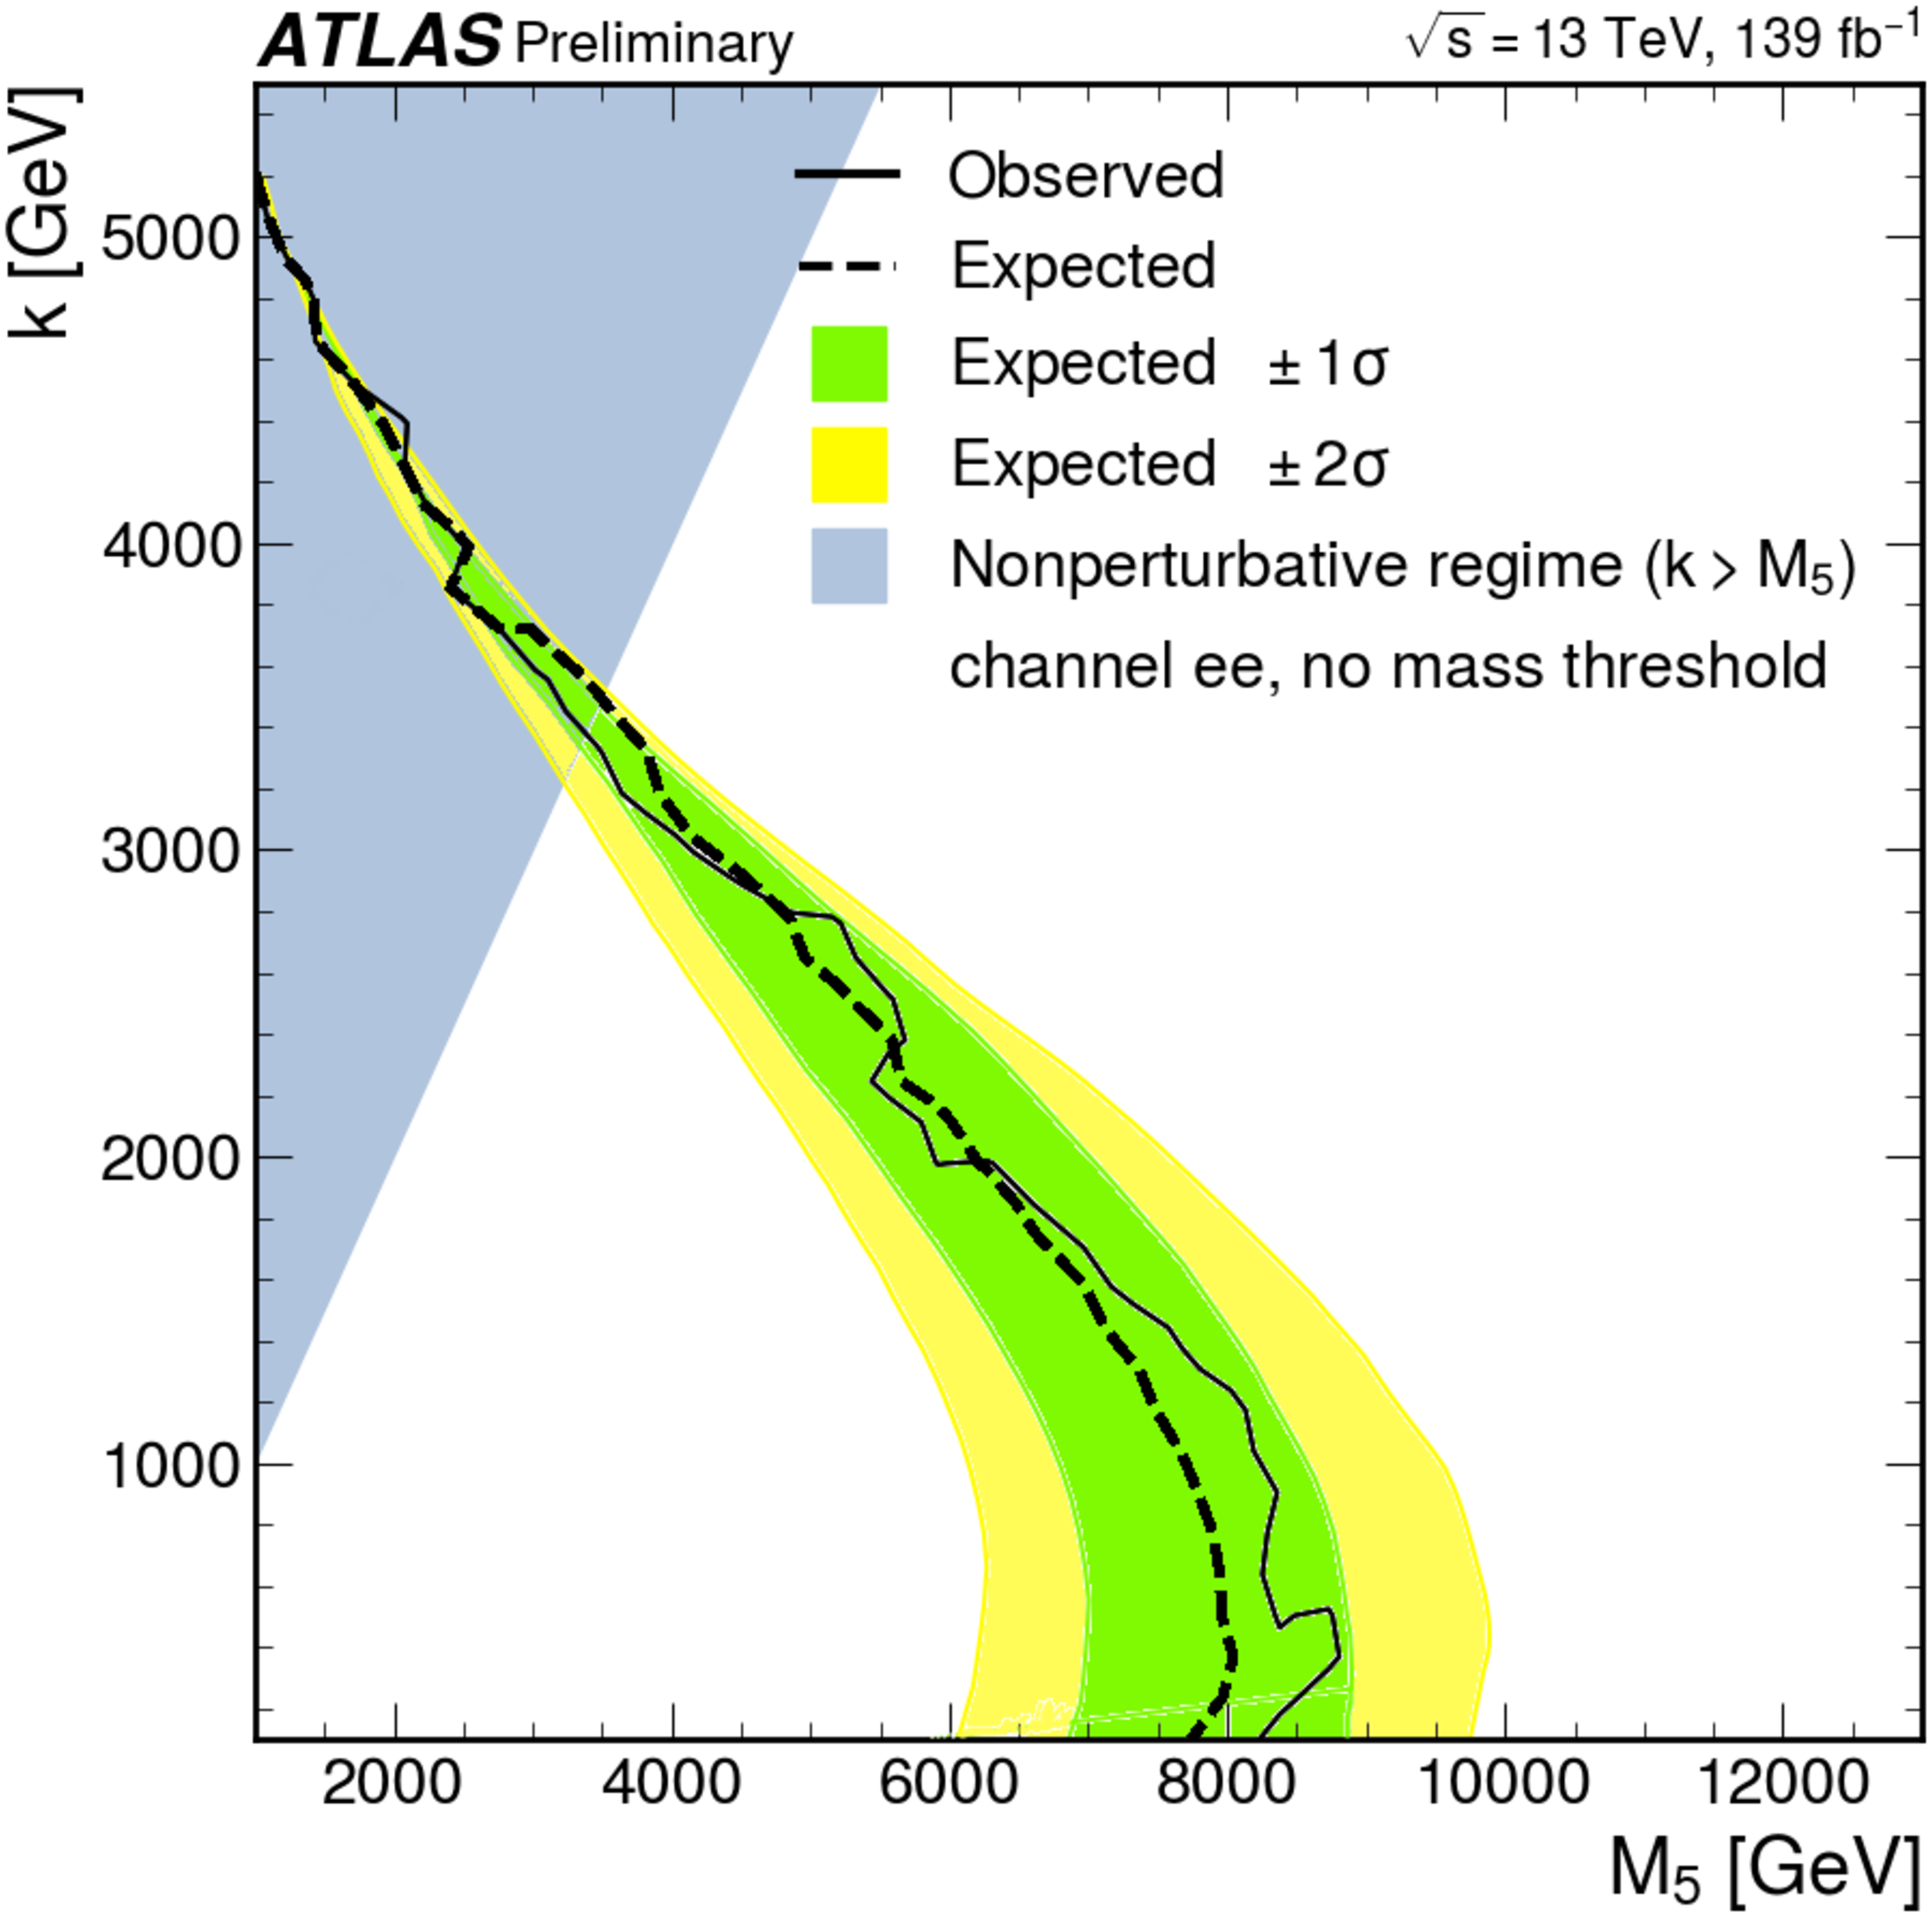
\includegraphics[width=\textwidth]{periodic}
         \caption{}
         \label{fig:perlimits}
     \end{subfigure}
        \caption{(a): The di-electron mass spectrum of a periodic signal. (b): Scalogram of a signal + background sample. (c): Observed (solid line) and expected (dashed line) limits on the model parameters, $M_{5}$ and $k$\protect\cite{period}.}
        \label{fig:periodic}
\end{figure}

\vspace{-0.5cm}

\section{Summary}

The search programme at ATLAS is expanding in multiple fronts. Advanced
detector performance and modern analysis techniques allow us to greatly enhance
the sensitivities. The unexplored regions and the gaps are being filled with
new searches applying unique search strategies. ATLAS is pioneering brand new
signature driven searches that challenge traditional methods vastly, motivating
us to think out of the box and experiment fresh new methodologies. In addition,
more effective theory interpretations are carried out in precision SM
measurements such as the lepton flavour violating top measurement~\cite{top}.
There are many interesting ongoing searches besides the ones covered in this
article, including exciting Run-3 results. More highlights are coming.       


\section*{References}

\begin{thebibliography}{99}

\bibitem{dijet} The ATLAS Collaboration, \Journal{\JHEP}{03}{145}{2020}.
\bibitem{vlq} The ATLAS Collaboration, ATLAS-CONF-2023-020, http://cds.cern.ch/record/2856892.
\bibitem{rhn} The ATLAS Collaboration, CERN-EP-2023-034, https://arxiv.org/abs/2304.09553.
\bibitem{tau} The ATLAS Collaboration, CERN-EP-2023-008, https://arxiv.org/abs/2303.09444.
\bibitem{bbyy} The ATLAS Collaboration, ATLAS-CONF-2023-009, http://cds.cern.ch/record/2854839.
\bibitem{micro} The ATLAS Collaboration, CERN-EP-2023-038, https://arxiv.org/abs/2305.02005.
\bibitem{dark} The ATLAS Collaboration, ATLAS-CONF-2023-016, http://cds.cern.ch/record/2855334.
\bibitem{tttt} The ATLAS Collaboration, CERN-EP-2023-048, https://arxiv.org/abs/2304.01678
\bibitem{clock} Gian F. Giudice and Matthew McCullough, \Journal{\JHEP}{02}{036}{2021}.
\bibitem{period} The ATLAS Collaboration, CERN-EP-2023-073, https://arxiv.org/abs/2303.09444.
\bibitem{top} The ATLAS Collaboration, ATLAS-CONF-2023-001, http://cds.cern.ch/record/2845451.

\end{thebibliography}

\end{document}

%%%%%%%%%%%%%%%%%%%%%%
% End of moriond.tex  %
%%%%%%%%%%%%%%%%%%%%%%


%%% Local Variables: 
%%% mode: latex
%%% TeX-master: t
%%% End: 

%%% Local Variables: 
%%% mode: latex
%%% TeX-master: t
%%% End: 

%%% Local Variables: 
%%% mode: latex
%%% TeX-master: t
%%% End: 
